%==============================================================================
% IEEE journal manuscript.
% Patient-Level Differential Privacy in Hierarchical Federated Learning for Multimodal Medical IoT
% (System name used in the body: PP-HFM.)
% Document class: IEEEtran (official).
%
% COMPILE THIS FILE. The files under sections/ are \section fragments: they
% carry no \documentclass and no \begin{document}, so compiling one directly
% gives "Undefined control sequence" at \section and a cascade of
% "Missing \begin{document}".
%   Overleaf: Menu -> Main document -> main.tex
%
% Build:  pdflatex main  ->  bibtex main  ->  pdflatex main  ->  pdflatex main
% (see README.md for a one-line latexmk command)
%==============================================================================
\documentclass[journal]{IEEEtran}

% ---- Packages --------------------------------------------------------------
\usepackage[T1]{fontenc}             % proper glyphs for accented names
\usepackage[utf8]{inputenc}          % input encoding (portable on older TeX)
\usepackage{cite}                    % IEEE-style reference handling
\usepackage{amsmath}                 % equations
\usepackage{amssymb}                 % math symbols
\usepackage{graphicx}                % figures
\graphicspath{{figures/}}            % figure search path
\usepackage{booktabs}                % professional tables (\toprule etc.)
\usepackage{array}                   % column formats (>{\raggedright} in the scope table)
\usepackage{multirow}                % multi-row table cells
\usepackage{algorithm}               % algorithm floats (Alg. 1, 2)
\usepackage{algorithmic}             % \STATE, \FOR, \REQUIRE inside them
\usepackage{stfloats}                % allow figure*/table* at page BOTTOM;
                                     % without it a double-column float may
                                     % only go to a page top, which is why
                                     % figure* drifts past its reference
\usepackage{url}
\usepackage[hidelinks]{hyperref}     % load last; internal/external links
\newtheorem{theorem}{Theorem}
\newtheorem{corollary}{Corollary}
\newtheorem{proposition}{Proposition}

% Improve display equation spacing for IEEE two-column layout
\setlength{\abovedisplayskip}{8pt plus 2pt minus 2pt}
\setlength{\belowdisplayskip}{8pt plus 2pt minus 2pt}
\setlength{\abovedisplayshortskip}{6pt plus 2pt minus 2pt}
\setlength{\belowdisplayshortskip}{6pt plus 2pt minus 2pt}

% ---- Front matter ----------------------------------------------------------
\begin{document}

\title{Patient-Level Differential Privacy in Hierarchical\\
       Federated Learning for Multimodal Medical IoT}

% (College grid) Authors as a grid under the title. Three columns of long e-mail addresses
% are wider than the page at the default author size; \small and tighter
% columns make the row fit.
% Author block: two layouts of the same authors.
%   \collegeauthorstrue  -> grid under the title (college format; default)
%   \collegeauthorsfalse -> IEEE journal format: names on one line, affiliation
%                           and e-mail in the first-page \thanks footnote, as the
%                           IEEE double-column journal template requires
%                           (IoT-J). ORCID iDs are entered in the submission portal.
\newif\ifcollegeauthors
\collegeauthorstrue
\ifcollegeauthors
\author{
{\small\setlength{\tabcolsep}{2pt}%
\begin{tabular}{ccc}
\begin{tabular}{c}
Samartha H V\\
\textit{Manipal Institute of Technology Bengaluru}\\
\textit{Manipal Academy of Higher Education}\\
Manipal, India\\
samartha1.mitblr2025@learner.manipal.edu
\end{tabular}
&
\begin{tabular}{c}
Shreyas J\\
\textit{Manipal Institute of Technology Bengaluru}\\
\textit{Manipal Academy of Higher Education}\\
Manipal, India\\
shreyas.j@manipal.edu
\end{tabular}
&
\begin{tabular}{c}
Udayaprasad P K\\
\textit{Manipal Institute of Technology Bengaluru}\\
\textit{Manipal Academy of Higher Education}\\
Manipal, India\\
udayaprasad.mitblr2024@learner.manipal.edu
\end{tabular}
\\ \noalign{\vspace{2.4em}}  % \\[len] is absorbed by the tall cells
\multicolumn{3}{c}{
\begin{tabular}{cc}
\begin{tabular}{c}
Shreelakshmi Yadav N\\
\textit{Manipal Institute of Technology Bengaluru}\\
\textit{Manipal Academy of Higher Education}\\
Manipal, India\\
shreelakshmi.mitblr2024@learner.manipal.edu
\end{tabular}
&
\begin{tabular}{c}
Sowmya T Rao\\
\textit{Manipal Institute of Technology Bengaluru}\\
\textit{Manipal Academy of Higher Education}\\
Manipal, India\\
sowmya.mitblr2024@learner.manipal.edu
\end{tabular}
\end{tabular}
}
\end{tabular}}\vspace{-2.6em}  % less space before the abstract
}
\else
\author{Samartha~H~V, Shreyas~J, Udayaprasad~P~K, Shreelakshmi~Yadav~N,
and Sowmya~T~Rao%
\thanks{The authors are with the Manipal Institute of Technology Bengaluru,
Manipal Academy of Higher Education, Manipal, India (e-mail:
samartha1.mitblr2025@learner.manipal.edu; shreyas.j@manipal.edu;
udayaprasad.mitblr2024@learner.manipal.edu;
shreelakshmi.mitblr2024@learner.manipal.edu;
sowmya.mitblr2024@learner.manipal.edu).}}
\fi

% Running head. \markboth takes TWO arguments; commenting out only the first
% line leaves the second as ORDINARY BODY TEXT, which prints a stray line and
% pushes the title onto page 2. Both lines are commented together, or neither.
% Uncomment and set the journal name once the venue is fixed.
%\markboth{IEEE Journal Name,~Vol.~XX, No.~XX, Month~2026}%
%{Author \MakeLowercase{\textit{et al.}}: Patient-Level Differential Privacy in Hierarchical Federated Learning for Multimodal Medical IoT}

\maketitle

% ---- Abstract & keywords ---------------------------------------------------
%==============================================================================
% abstract.tex — FINAL. Supersedes the placeholder; abstract_draft.tex is its
% ancestor and is kept only for its provenance notes.
%
% TITLE IS FIXED. The abstract's job is to EARN each element of it, and one
% element is earned CONDITIONALLY and must stay that way:
%
%   HIERARCHICAL  — three tiers, edge tier INSIDE the privacy accounting.
%                   O1 90.822% / 96.082%, O4 72.300% / 76.841%. Collapsing the
%                   tier does NOT improve accuracy (A1-A0 = -0.0047 / -0.0052
%                   at n=6), so the savings cost no utility. Do NOT upgrade
%                   this to "the hierarchy improves accuracy": the flat arm
%                   also drops from five edge rounds to one, so topology and
%                   aggregation schedule are confounded.
%   PRIVACY-AWARE — patient unit by construction; composed eps 0.970 / 0.966
%                   INCLUDING the conformal quantile; MIA audit with a passing
%                   positive control (0.625 on a memorizing configuration).
%   LOW-LATENCY   — O3a P95 2.299 ms / 0.754 ms (1000-run bench, FP32). Quote THIS. Never quote
%                   absolute round latency: its compute terms are analytical.
%   MULTIMODAL    — paired at source, and a CONDITIONAL result. +0.0370 AUROC
%                   on vitaldb; wear cannot test it (best single 0.9976);
%                   eICU is a NULL (+0.0037 AUROC, -0.0001 AUPRC) AND HAS MORE
%                   HEADROOM THAN VITALDB (0.1788 vs 0.1717) — so the eICU null
%                   is NOT explained by a ceiling. The earlier draft said
%                   "nothing where one modality already suffices", which is
%                   true of wear and FALSE of eICU. Never claim an
%                   unconditional fusion benefit.
%   IoT SYSTEMS   — packet-level NS-3, CloudSim energy, ONNX deployment.
%   THREE DEPLOYMENTS (2026-10-22): eICU adds eps 0.834, O1 92.3 %, O4 79.6 %,
%                   O3a 0.24 ms, so every bound quoted in the body sentence
%                   ("at least 90.8 / 72.3 %", "at most 2.3 ms", eps <= 1) holds
%                   on all three. eICU O3b FAILS (97.83 %) and O2b is
%                   inconclusive: neither is claimed here, so do not add
%                   delivery or accuracy to that sentence.
%
% LENGTH: 249 words in the rendered PDF, inside the ~250 cap IEEE TII and
% IoT-J apply. Measure it from `pdftotext` in READING ORDER, not with
% -layout: -layout interleaves the two columns and reports ~462.
%
% Trimmed 2026-10-19 from 302. Every finding and every headline number was
% kept; what went was connective prose, the second of each paired percentage
% (now "at least X" -- uplink is 90.8/96.1, energy 72.3/76.8), and the
% restatement of the metric in the fusion clause, which the preceding
% sentence already establishes as area under the ROC curve.
%
% Keywords live in main.tex, not here — two IEEEkeywords blocks is an error.
%==============================================================================

\begin{abstract}
Hierarchical federated learning keeps Internet-of-Things data local, but its differential-privacy guarantee protects single
records, whereas clinical deployments must protect patients, each with many
records. This paper proposes PP-HFM, a client--edge--cloud framework whose
privacy unit is the patient. Each client clips a patient's summed gradient,
calibrates noise to its population and accounts for every hierarchical
release. The guarantee is proved for the training transcript and holds end to
end with public encoders and standardization constants (eICU). PP-HFM is evaluated on
VitalDB, an eICU cohort of $187$ hospitals and, at record level, a wearable
corpus. At a training budget of at most
$\varepsilon = 0.9$ ($1.0$ with an evaluated conformal release; $0.766$ at
record level on WEAR), it reduces
uplink traffic by $90.8$--$96.1\,\%$ and modeled energy per round by
$72.3$--$79.6\,\%$; $95$th-percentile inference latency on a workstation CPU
is at most $2.3$~ms. On VitalDB, partitioned by person, the guarantee costs no
utility (area under the ROC curve, AUC, $0.832$ against $0.820$ non-private); on
eICU it costs $3.1$ points (inconclusive against the two-point target) and
$3.9$ end to end, which misses it; non-private HED-FL is more accurate
($0.825$ against $0.794$). PP-HFM
uploads $2.2$--$4.0$ times less than re-implemented HED-FL and FL2DP and shows
lower measured leakage than both in the VitalDB audit. On VitalDB and WEAR, pretrained initialization,
not head-only noise,
makes a strict budget survivable; the cost of the patient unit follows
$A(1 - 1/k)$ in records per patient $k$. A VitalDB membership-inference audit
with a positive control finds record-level training above its difficulty floor
(likelihood-ratio attack AUC $0.576$) and patient-level training at it
($0.503$).
\end{abstract}


\begin{IEEEkeywords}
Hierarchical federated learning, Internet of Things, differential privacy,
user-level privacy, membership inference, multimodal learning, edge computing,
quality of service, conformal prediction, clinical decision support.
\end{IEEEkeywords}

\IEEEpeerreviewmaketitle

% ---- Body (one file per section) -------------------------------------------
% All body sections are drafted and included. The abstract still points at
% sections/abstract.tex; sections/abstract_draft.tex is the proposed
% replacement and the swap is an editorial decision, not made here.
%==============================================================================
% introduction.tex — Introduction for PP-HFM
% Self-contained \section{}; \input this into main.tex (never compile alone).
%
% Structured after the house introduction template: domain motivation, the
% task, what makes it hard, how approaches developed, what each leaves open,
% the remedies that follow, "Accordingly, this work...", an enumerated
% contribution list with explicit non-claims, and the organisation paragraph.
%
% POSITIONING RULE (docs/roadmap.md): user-level DP, parameter-efficient DP
% fine-tuning and DP quantile release are PRIOR ART. The contributions are
% measurements and auditing practice. Do not write "we propose patient-level
% DP".
%
% NOTE: the contribution list covers only completed work. The records-per-
% individual scaling law completed 2026-08-16 (24/24 configurations) and is
% now the fifth contribution; see Sec. Results, "Records per individual".
% It is stated in AUPRC only -- the AUROC trend is monotone in the same
% direction but every interval covers zero at three seeds, so it is reported
% as directionally consistent and not as a resolved effect.
%==============================================================================

\section{Introduction}
\label{sec:intro}

Internet-of-Things deployments increasingly derive their value from combining
sensing streams of different kinds. A hospital theatre records continuous
physiological waveforms alongside the structured clinical history of the
patient on the table; a wearable installation records inertial motion alongside
egocentric video. In each case the streams are complementary rather than
redundant, and a model with access to both can resolve states that neither
resolves alone. The streams are also produced where the sensors are, which is
seldom where computation is convenient, and this tension between where data
arises and where models are trained is the setting the present work addresses.

Transmitting raw multimodal streams to a central service is the obvious
resolution and is frequently unavailable. The volume is substantial and the
uplink is the scarce resource, so centralisation inflates both latency and
energy in precisely the deployments that can least afford either. More
decisively, in the settings where multimodal sensing is most valuable the data
cannot lawfully move at all: clinical records are governed by consent and by
data-protection regimes that prohibit pooling across institutions, so a model
requiring centralisation cannot be deployed rather than merely being expensive.
Federated learning \cite{ref1} answers this by communicating model updates
instead of records, and hierarchical variants \cite{ref2, ref3} interpose an
edge tier so that the wide-area link is exercised once per several local
rounds.

Moving the model rather than the data does not by itself protect the data. The
updates a client transmits are functions of its records, and membership
inference against released models is well established \cite{ref14}. A formal
guarantee is therefore required, and differentially private stochastic gradient
descent \cite{ref6} supplies one by bounding the influence of a training record
and perturbing the aggregate. But the guarantee such a system reports is stated
over the unit it clips, and in a sensing deployment that unit is a
fixed-length window rather than a person. Where an individual contributes many
windows --- as every patient does, and as every participant in a continuous
recording does --- a record-level budget answers whether a particular window
was used in training, while the question a clinical deployment must answer is
whether a particular \emph{person} was. The two can be related by group
privacy \cite{ref8}, but at the group sizes these datasets exhibit the
conversion is prohibitive, turning a nominal budget of unity into one that
supports no meaningful claim.

Existing systems have developed along two lines that do not meet. Hierarchical
designs establish the communication and energy case convincingly: HED-FL
\cite{ref3} extends deployment lifetime by avoiding long-range transmission,
HCEF \cite{ref4} adapts computation and compression to device heterogeneity,
and assignment-oriented work \cite{ref5} reduces divergence under non-identical
distributions. None carries a formal privacy guarantee. Private designs supply
the guarantee: FL2DP \cite{ref9} couples noise with shuffling, and RoPPFL
\cite{ref10} pairs local privacy with robust aggregation at the edge. Neither
is hierarchical in the sense that matters here, and neither examines how an
intermediate tier alters the frequency with which each client's budget is
spent. Across both lines the local objective is treated as the aggregation of
generic parameter vectors, so neither multiple modalities per record nor the
grouping of records under an individual plays any part.

Three difficulties follow, and they bear on deployability as much as on
privacy. The unit at which a guarantee is stated is rarely examined, so its
cost on genuinely paired multimodal data is unquantified. The validity
condition of parameter-efficient private training --- that the corpus used to
pretrain the frozen representation be disjoint from the protected population
\cite{ref12, ref13} --- is frequently left implicit and, where honoured,
unpriced. And guarantees are typically reported from the parameters of the
mechanism rather than audited by attack; where an audit is performed it is
conducted at the granularity of the record, which is precisely the quantity a
record-level guarantee already protects.

Two remedies follow directly. The unit can be fixed at the point of clipping
rather than recovered afterwards by a group-privacy conversion: if the
gradients of an individual's records are accumulated before the bound is
applied, that individual's influence on the released model is bounded
irrespective of how many records they contributed, and accounting performed at
the same granularity yields a budget that is a statement about people by
construction. And the resulting guarantee can be audited by mounting membership
inference at the level of the individual, provided the attack used is strong
enough that a negative finding is informative --- which requires demonstrating
on a configuration known to memorise that the attack can find leakage where
leakage exists.

Accordingly, this work presents PP-HFM, a three-tier federated framework for
multimodal sensing in which the privacy unit is the individual by construction.
Records are grouped by individual before they are bounded; the noise scale is
calibrated to satisfy the budget for every client simultaneously rather than
for a representative one, so that the interposition of the edge tier is
reflected in the reported figure; and the cost of releasing a conformal
calibration quantile is composed into that figure rather than omitted from it.
Representation learning is separated from private adaptation, with encoders
pretrained on a population disjoint from every client and frozen, so that only
a compact fusion head is privatised. The framework is evaluated on two corpora
whose modalities are associated by the recording apparatus rather than by a
construction rule, under a protocol that measures communication, latency,
reliability and energy on a simulated topology and audits the privacy guarantee
by attack.

The contributions are fivefold. First, the framework enforces an
individual-level guarantee within a hierarchical multimodal system and reports
a composed budget covering both training and calibration; the accounting
practices this requires --- calibrating the noise against every client rather
than a representative one, and charging the calibration release against the
same budget --- are specified in enough detail to be checked from outside,
because each corresponds to a failure that is invisible in a training log.
Second, the cost of the choice of unit is measured on genuinely paired clinical
multimodal data, together with the cost of the disjointness condition that
makes the guarantee valid end-to-end, so that both are priced rather than
assumed negligible. Third, the guarantee is audited by patient-level membership
inference under both a threshold attack and a likelihood-ratio attack
\cite{ref17}, each reported alongside a positive control on a configuration
known to memorise; the audit returns a null on the private arms, and the
control is what makes that null attributable to the defence rather than to an
inadequate adversary. Fourth, the system-level behaviour is validated on two
deployments differing in topology and in payload, with every network quantity
measured on rounds in which the payload traversed the simulated topology rather
than composed analytically. The same protocol establishes that the guarantees
are affordable in real time: the conformal set construction that carries the
coverage guarantee occupies $0.68\,\%$ of the inference path, and the private
mechanism occupies none of it, since its noise is applied to gradients during
training and adds no operation to serving. The objection that a privacy
apparatus is too heavy for a latency-bound deployment is therefore answered by
measurement rather than by argument. Fifth, the price of the individual-level guarantee
is shown not to be a fixed quantity but a function of how much each individual
contributes: with the per-step budget and the number of units per step held
constant, the penalty is indistinguishable from zero when an individual
contributes a single record and grows monotonically as that number rises,
saturating by eight records. This design carries its own control, because at one
record per individual the two units coincide by construction and the two arms
must agree; that they do is what licenses reading the divergence at larger
contributions as a property of the unit rather than of the apparatus.

What is not claimed should be stated as plainly. User-level differential
privacy \cite{ref11}, parameter-efficient differentially private fine-tuning
\cite{ref12, ref13} and differentially private quantile release \cite{ref24}
are established prior art, and are used here rather than proposed. The
contributions above are measurements of these mechanisms in a setting where
they have not been measured, and the auditing practice under which those
measurements are reported.

The remainder of the paper is organised as follows. Section~\ref{sec:related}
reviews related work on hierarchical and private federated learning, on the
unit at which a guarantee is stated, and on membership inference as an
auditing instrument; Section~\ref{sec:method} presents the proposed framework;
Section~\ref{sec:experiments} specifies the corpora, the implementation, the
evaluation measures and the experimental protocol; Section~\ref{sec:results}
reports the results; Section~\ref{sec:discussion} discusses their
interpretation and the limitations of the study; and
Section~\ref{sec:conclusion} concludes.

%==============================================================================
% related_work.tex — Related Work for PP-HFM
% Self-contained \section{}; \input this into main.tex (never compile alone).
%
% Structured after the house related-work template: one dense paragraph per
% subsection, each closing on the limitation that motivates the next, and a
% final Summary and Research Gap that enumerates the observations before
% stating how the present work addresses them.
%
% POSITIONING RULE (non-negotiable, see docs/roadmap.md):
%   Claim: "we quantify what has not been quantified, and audit it properly."
%   NOT:   "we invented patient-level DP."  <- desk reject
% User-level DP (McMahan 2018), parameter-efficient DP fine-tuning (Li 2021,
% Yu 2021) and DP quantile release (Smith 2011) are PRIOR ART and are named as
% such before any gap is claimed.
%==============================================================================

\section{Related Work}
\label{sec:related}

\subsection{Federated Learning and Hierarchical Aggregation}

The formulation of distributed training as the communication of model updates
rather than of data \cite{ref1} established the basis upon which
subsequent federated systems were constructed. In its flat form, however, every
participating client transmits to a central server in every round, so that the
wide-area link rather than local computation determines how frequently the
global model may be revised. Client--edge--cloud designs \cite{ref2}
addressed this by interposing an intermediate tier at which several rounds of
local optimisation are absorbed before one round of central aggregation is
performed. HED-FL \cite{ref3} developed the principle for
constrained deployments, clustering devices dynamically at the edge and
demonstrating that the avoidance of long-range transmission substantially
extends the operational lifetime of an installation, while HCEF
\cite{ref4} introduced heterogeneity awareness, adjusting per-device
computation frequency and compression ratio online so that the slowest
participant does not dictate the duration of a round. Mhaisen \emph{et al.}
\cite{ref5} treated the assignment of clients to aggregators as
the object of optimisation, showing that an assignment informed by the
statistical properties of local data reduces model divergence under
non-identically distributed conditions. These works establish the
communication and energy case for hierarchy convincingly, and the present study
adopts rather than re-derives it. None of them, however, carries a formal
privacy guarantee: HED-FL provides none, and the assignment strategy of
\cite{ref5} requires clients to disclose local label
statistics, which is itself a release of information about the protected
population and is difficult to reconcile with a strict budget.

\subsection{Differential Privacy in Federated Learning}

Differentially private stochastic gradient descent \cite{ref6}
supplies the guarantee that hierarchical designs omit, bounding the influence of
a training record by clipping its gradient to a fixed norm and perturbing the
aggregate with calibrated noise, with the accumulated cost tracked by a moments
or R\'enyi accountant \cite{ref7} within the framework of
\cite{ref8}. Within federated learning the mechanism has been
developed in two principal directions. FL2DP \cite{ref9} combines an
exponential noise mechanism with a shuffling entity that severs the association
between a client and the update it contributes, reporting improved accuracy at
an equivalent formal guarantee, while RoPPFL \cite{ref10} pairs local
differential privacy with similarity-based robust aggregation performed at the
edge, so that the intermediate tier serves as a verifier against corrupted
updates as well as a relay. Both establish that a formal guarantee is
attainable in the federated setting at acceptable cost. Both, however, are
organised flatly with respect to the property considered here: FL2DP provides
differential privacy without a hierarchy in the sense that the edge tier plays
no part in the accounting, and neither examines how the interposition of such a
tier alters the frequency with which each client's budget is expended, which is
the quantity upon which the calibration of the noise ultimately depends.

\subsection{The Unit to Which a Guarantee Attaches}

The distinction between a guarantee stated over records and one stated over
individuals is long established and is not a contribution of the present work.
McMahan \emph{et al.} \cite{ref11} introduced user-level
differential privacy for federated language models, bounding the contribution of
each user rather than of each example, and the group-privacy relation by which
one may be converted into the other is standard \cite{ref8}.
The mechanism is therefore available; what is not available is a measurement of
what it costs in the setting that most requires it. In clinical monitoring the
grouping of records under an individual is not a property of a few atypical
participants but of every participant, since a single episode of care yields
many time-aligned records, and the conversion factor is consequently applied to
the whole population rather than to its tail. The literature supplies neither
the utility forgone when the unit is moved from the record to the individual on
genuinely paired multimodal clinical data, nor the manner in which that cost
varies with the number of records an individual contributes, and in the absence
of the latter a single measurement cannot be distinguished from a property of
the particular cohort on which it was obtained.

\subsection{Parameter-Efficient Private Adaptation}

The perturbation that a parameter vector must absorb under a fixed budget grows
with its dimensionality, so that private training of an entire network degrades
severely at the budgets a clinical claim requires. Restricting the private
optimisation to a compact trainable subset situated above frozen pretrained
representations is an established remedy, and Li \emph{et al.}
\cite{ref12} and Yu \emph{et al.} \cite{ref13} demonstrate
that parameter-efficient differentially private fine-tuning is markedly more
robust at small $\varepsilon$ than end-to-end private training. The present
work adopts this recipe and claims no novelty for it. The recipe nevertheless
carries a precondition that is frequently left implicit: the corpus upon which
the frozen representations are obtained must be disjoint from the protected
population, since otherwise the representations have already been derived from
that population without a guarantee and the budget subsequently reported for
the trainable component does not describe the system as a whole. Where the
precondition is honoured it is seldom priced, so the utility conceded in order
to obtain a guarantee that is valid end-to-end remains unquantified; and the
consequences of the recipe for what the resulting model retains of its training
population have received little attention.

\subsection{Membership Inference as Empirical Auditing}

A differential privacy guarantee is an upper bound upon the influence of a
participant and does not by itself establish what an adversary attains in
practice, for which membership inference supplies the complementary
measurement. Shokri \emph{et al.} \cite{ref14} introduced the
shadow-model formulation, and thresholding of the loss or confidence
\cite{ref15} remains the most commonly reported attack. Such
attacks are weak by construction: a single global threshold is confounded by
the varying difficulty of individual examples, so that an easily fitted
non-member may be scored above a poorly fitted member and the reported strength
constitutes a lower bound upon leakage rather than an estimate of it. Watson
\emph{et al.} \cite{ref16} demonstrated that calibrating against
per-example difficulty alters conclusions materially, and Carlini \emph{et al.}
\cite{ref17} formalised the calibration as a likelihood-ratio test
between per-example in- and out-distributions estimated from shadow models,
arguing further that attacks should be assessed by their true-positive rate at
low false-positive rate rather than by an average-case summary that conceals
confident identification of a minority. Two limitations persist. Membership is
almost invariably evaluated at the granularity of the training record, which is
precisely the quantity that a record-level guarantee already protects and not
the quantity a clinical guarantee concerns; and negative results are rarely
accompanied by evidence that the attack employed was capable of a positive one,
so that an absence of detected leakage cannot be distinguished from an
inadequate adversary.

\subsection{Multimodal and Clinical Federated Learning}

The motivation for federated learning is particularly clear in medicine, where
governance rather than volume prevents the assembly of data at a single site
\cite{ref18, ref19}. The majority of federated work,
including the systems discussed above \cite{ref9, ref3, ref4, ref10}, nevertheless treats the local objective as the
aggregation of generic parameter vectors and does not represent multiple
modalities per record, notwithstanding that clinical evidence is characteristically
multimodal and that the modalities available at one institution may differ from
those available at another. Where multimodal federated benchmarks have been
assembled, the modalities are frequently associated by a construction rule
rather than by common provenance, so that an apparent benefit of fusion may
reflect the regularity of the rule rather than genuinely complementary
information; a benchmark of this kind cannot support a claim about fusion at
all. Corpora in which both modalities originate from the same individual during
the same episode and are aligned at the point of capture
\cite{ref20}, or are synchronised in hardware
\cite{ref21}, avoid the difficulty entirely, since the association is a
property of the source and requires no defence.

\subsection{Uncertainty Quantification under a Privacy Budget}

Conformal prediction provides prediction sets carrying a distribution-free
coverage guarantee and requires neither retraining nor distributional
assumptions \cite{ref22, ref23}, which
recommends it for clinical deployment, where a point prediction unaccompanied
by a statement of confidence is of limited use. Its application within a
private system introduces a complication that is easily overlooked: the
procedure requires the release of a quantile of nonconformity scores computed
upon held-out data belonging to the protected population, and such a release is
a disclosure in exactly the sense the surrounding framework exists to bound.
Differentially private release of a quantile by the exponential mechanism is
itself standard \cite{ref24}, so the mechanism is not at issue.
What is at issue is the accounting: the cost of calibration composes with the
cost of training, and a system that reports only the latter understates the
budget it has expended, by a factor that grows with the number of occasions on
which calibration is performed.

\subsection{Real-Time Inference and Quality of Service at the Edge}

A federated system is trained once and queried continuously, and the constraint
that governs its clinical usefulness after deployment is the delay between a
measurement arriving and a decision being available, rather than the time taken
to reach convergence. The federated literature has addressed the latter
extensively and the former hardly at all: HCEF \cite{ref4} adapts computation
frequency and compression ratio online, but the quantity it optimises is the
duration of a training round; RoPPFL \cite{ref10} places verification at the
edge in order to reject corrupted updates, prioritising robustness over
response time; and HED-FL \cite{ref3} is concerned with the energy consumed in
reaching a model rather than the latency of using one. Where inference cost has
been considered it has generally been within the edge-computing literature
rather than the federated one \cite{ref25}, and the principal instrument is
reduced-precision arithmetic, integer quantisation in particular being well
established as a means of lowering both memory footprint and inference time on
commodity hardware \cite{ref26}. The consequence is a gap that matters
precisely for the systems this work targets: a federated design may satisfy a
strict privacy budget and still be unusable at the bedside if the delay between
observation and prediction exceeds the window in which a clinician can act,
and no existing federated system reports an end-to-end inference latency
measured under the privacy mechanism it deploys, alongside the communication
and energy costs incurred in producing the model that serves it.

\subsection{Summary and Research Gap}

These lines of work converge upon the setting from which the present study
proceeds, and five observations remain. First, hierarchy and formal privacy
have been developed largely in separation --- the hierarchical systems provide
no guarantee, and the private systems do not examine how an intermediate tier
alters the expenditure of the budget --- so that the interaction between the two
is unmeasured although each is individually well understood. Second, the
mechanism for stating a guarantee over individuals rather than records is
established, but its cost on genuinely paired clinical multimodal data is not,
and in the absence of any characterisation of how that cost varies with the
number of records an individual contributes, a single measurement cannot be
distinguished from an artefact of the cohort upon which it was obtained. Third,
parameter-efficient private adaptation is widely adopted, yet the disjointness
of the pretraining corpus upon which its validity depends is frequently left
implicit and, where honoured, is not priced. Fourth, guarantees are typically reported from the parameters of the mechanism
rather than audited by attack; where an audit is conducted it is performed at
the granularity of the record, and a null result is seldom accompanied by the
evidence that would distinguish an effective defence from an inadequate
adversary. Fifth, and cutting across the foregoing, the cost of a federated
design is reported in the currency of training --- rounds to convergence,
bytes exchanged, energy expended --- while the delay experienced by the
clinician who queries the deployed model is left unmeasured, notwithstanding
that it is this delay which determines whether the system can be used at the
point of care at all.

The present work addresses these five points together. It combines a two-tier
hierarchy with a guarantee whose sensitivity is enforced at the level of the
individual at the point of clipping rather than recovered by conversion
afterwards, and calibrates the noise against every client simultaneously so
that the interposition of the edge tier is reflected in the reported budget. It
measures the utility conceded by moving the unit from the record to the
individual, and characterises that cost as a function of the number of records
each individual contributes rather than at a single operating point. It
enforces and verifies the disjointness of the pretraining population, and
reports the utility forgone in order that the resulting guarantee be valid
end-to-end. Finally, it audits the guarantee by mounting membership inference
at the level of the individual, using both a threshold attack and a
likelihood-ratio attack calibrated per individual, and reports every result
alongside a positive control on a configuration known to memorise, so that a
negative finding may be attributed to the defence rather than to the adversary.
Finally, it specifies and instruments the deployment path, so that the
end-to-end latency of a prediction, the volume of traffic the hierarchy
carries, and the energy each tier expends are reported for the same
configuration that carries the privacy guarantee, rather than for a
differently-configured system.

%==============================================================================
% method.tex — Methodology for PP-HFM
% Self-contained \section{}; \input this into main.tex (never compile alone).
%
% Structured after the house methodology template: domain motivation, then a
% blueprint subsection, then one subsection per component (motivation ->
% description -> placement -> transition), with every equation gathered into a
% final formulation subsection.
%
% Required in the host preamble:
%   amsmath, amssymb, booktabs, algorithm, algorithmic, graphicx
% READABILITY PASS 2026-10-21: formal register; inter-subsection transitions
% removed; misplaced group-privacy sentence restored to its paragraph; the
% wrong forward reference before the deployment subsection fixed. Floats and
% equations are copied verbatim.
%==============================================================================

\section{Methodology}
\label{sec:method}

\subsection{Problem Statement}
\label{sec:method:problem}

Multimodal Internet-of-Things deployments combine sensing streams of different
kinds, such as physiological monitors with clinical records or inertial sensors
with video, at the location where the streams are produced. The training data
are therefore distributed, and in clinical settings they cannot be centralized,
because consent and data-protection regulations prohibit pooling. Federated
learning addresses this by moving the model instead of the data, but it does
not provide a privacy guarantee, because client updates are functions of the
client's records. A suitable framework must therefore combine distributed
multimodal training with a formal guarantee, within the network, latency and
energy constraints of an edge installation.

Differentially private federated learning provides such a guarantee, but the
\emph{unit} of the guarantee in clinical settings has received little
attention. Standard differentially private stochastic gradient descent
\cite{ref6} clips and accounts per training record. In a monitoring dataset, a
record is a fixed-length window rather than a person, and every patient in the
cohort used here contributes several windows. A record-level budget therefore
bounds whether a particular window was used in training, whereas a clinical
guarantee must bound whether a particular \emph{patient} was. Prior federated
systems address only one side of this problem. HED-FL \cite{ref3} provides a
hierarchical tier without differential privacy, FL2DP \cite{ref9} provides
differential privacy without a hierarchy, and neither these nor the
heterogeneity-aware and assignment-oriented designs \cite{ref4, ref5} model
multiple modalities per record or the grouping of records by individual.

The problem addressed is therefore the following. Several institutions each
hold multimodal recordings of their own patients, every patient contributes
many records, and no record may leave its institution. A shared model must be
trained through a client--edge--cloud hierarchy such that
\begin{enumerate}
\item the participation of any single patient, with all of their records, is
protected by a formal $(\varepsilon,\delta)$ guarantee that covers every
message the system releases, edge tier included;
\item the model remains close in utility to an identical non-private system;
and
\item the system remains deployable on IoT infrastructure, with low uplink
traffic, reliable delivery, low inference latency and low energy.
\end{enumerate}
These requirements interact. Protecting patients instead of records reduces
the number of protected units and therefore raises the relative noise;
clients partitioned by institution differ greatly in size, so a noise level
fitted to the smallest client degrades every larger one; and an edge tier
changes how many optimization steps each client takes, and hence how much of
its budget it spends. Table~\ref{tab:objectives} turns the three requirements
into seven quantitative targets, fixed before any experiment was run.

\subsection{Overall Framework of the Proposed PP-HFM}
\label{sec:method:overview}

This work therefore proposes a framework in which the privacy unit is the
patient by construction, and in which the hierarchy and the guarantee are
designed jointly. The system, PP-HFM (Patient-Private Hierarchical Federated
Multimodal learning), has three tiers: institutional clients that hold
patient-grouped multimodal records and never release them, edge aggregators
that perform several local rounds before communicating upward, and a cloud
aggregator that maintains the global model. Within each client, representation
learning is separated from private adaptation. Encoders pretrained on a
disjoint public population are frozen, and only a compact fusion head is
trained under a differentially private objective with patient-level
sensitivity. Fig.~\ref{fig:pphfm_arch} shows the overall organization.

\begin{figure*}[!t]
\centering
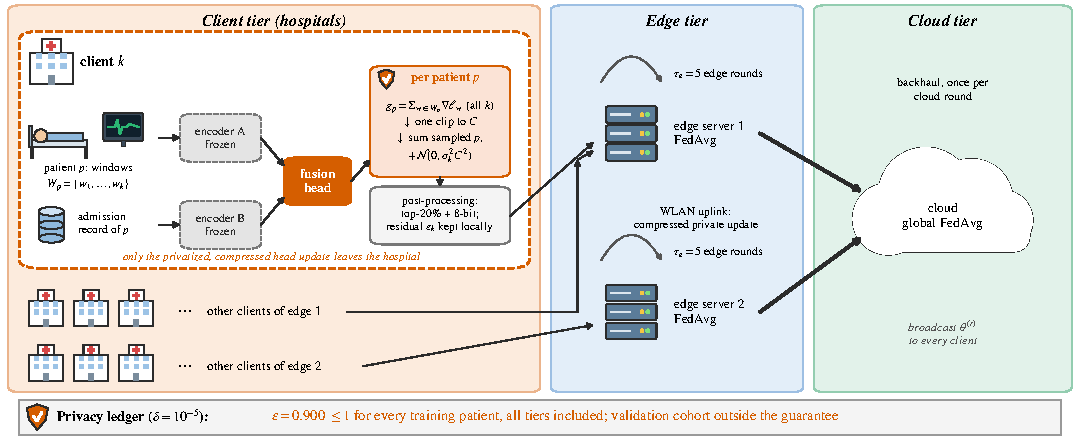
\includegraphics[width=\textwidth]{fig01_overview_core.pdf}
\caption{Architecture of PP-HFM. Each institutional client holds
patient-grouped multimodal records that never leave the institution, runs
frozen pretrained encoders, and privately trains only the fusion head, with
gradients summed per patient before clipping. Two edge aggregators perform
$\tau_e$ rounds of weighted averaging for every cloud round, and the cloud
averages the noisy, compressed updates globally.}
\label{fig:pphfm_arch}
\end{figure*}

Each client samples a batch of patients rather than windows, sums the
gradients of all windows of each sampled patient into one per-patient
gradient, clips that gradient, and adds noise to the aggregate once per
optimization step. The influence of any individual on the released model is
therefore bounded regardless of the number of records contributed. The
resulting update is compressed and sent to the client's edge, which averages
the updates of its clients. After several edge rounds, the edges report to the
cloud, which averages across edges and redistributes the global model.

The framework comprises the following components, each described in one of
the following subsections.
\begin{enumerate}
\item \emph{Frozen multimodal backbone} (Section~\ref{sec:method:backbone}):
fixed encoders, one per modality, and a compact trainable fusion head.
\item \emph{Patient-level privacy mechanism}
(Section~\ref{sec:method:privacy}): enforces sensitivity with respect to the
individual.
\item \emph{Noise calibration across clients}
(Section~\ref{sec:method:calib}): meets the budget for every client despite
large differences in client size.
\item \emph{Two-tier aggregation} (Section~\ref{sec:method:agg}): produces
the global model while using the wide-area link once per several local rounds.
\item \emph{Update encoding} (Section~\ref{sec:method:encoding}): reduces the
transmitted payload.
\item \emph{Deployment path} (Section~\ref{sec:method:deploy}): executes the
released model within a latency budget.
\item \emph{Network and energy instrumentation}
(Section~\ref{sec:method:instr}): measures the communication and energy costs
of the hierarchy.
\item \emph{Empirical audit} (Section~\ref{sec:method:mia}): tests the
resulting guarantee by membership inference.
\end{enumerate}
The encoder architecture and the aggregation rule
are adopted from established work and are not claimed
as contributions.

\subsection{Overall System Architecture}
\label{sec:method:arch}

PP-HFM is a three-tier federated system built on a frozen multimodal backbone.
Responsibilities are separated: the encoders provide fixed representations, a
compact head contains all trainable and privatized parameters, an edge tier
absorbs local rounds to reduce wide-area traffic, and a cloud tier maintains
the global model. The encoder design and the weighted averaging rule are
adopted from prior work. The design
contribution lies in the unit at which privacy is enforced and in the
accounting of the reported budget.

The architecture is shown in Fig.~\ref{fig:pphfm_arch}. An institutional
client holds a set of patients, each contributing several time-aligned
multimodal records. The records are encoded by two frozen modality-specific
encoders and combined by a trainable fusion head. The head is optimized under
a differentially private objective, and its compressed update is the only
quantity that leaves the institution. Updates are averaged at the edge over the
clients it serves. After $\tau_e$ such rounds, the edge models are averaged at
the cloud and redistributed. No record, single-record gradient or uncompressed
update crosses an institutional boundary.

The system consists of three functional groups. The first is the frozen
backbone: two modality-specific encoders, pretrained on a population disjoint
from every federated client and not adapted during federated training. The
second is the privatized trainable component: the fusion head, the
patient-level clipping and noise mechanism that governs its optimization, and
the calibration procedure that sets the noise scale. The third comprises the
communication components: the update encoding and the two-tier averaging.

Information flows in a group-then-bound structure. Within a client, records
are encoded and combined by the head, and gradients are grouped \emph{by
patient} before clipping, so that the clipped quantity is a patient's total
contribution rather than a single record's. Noise is added once to the
aggregate of the clipped per-patient gradients, after which the update is
compressed and transmitted. Communication is hierarchical: client to edge in
every edge round and edge to cloud once per cloud round, with the ratio set by
$\tau_e$.

This design follows from the constraints of the setting. Grouping gradients by
patient before clipping makes the guarantee a statement about individuals, and
avoids the severe degradation of a group-privacy conversion. Restricting
private optimization to a small head over frozen features keeps the dimension
of the perturbed vector low, which is necessary for acceptable utility under a
tight budget. Pretraining the features on a disjoint population keeps the
guarantee valid end to end. The edge tier reduces wide-area transmissions by a
factor of $\tau_e$ without changing the learning objective. Because the
encoders are fixed and the aggregation rule is standard, observed differences
can be attributed to the privacy unit and its accounting rather than to the
representation or the averaging.

\subsection{Frozen Multimodal Backbone}
\label{sec:method:backbone}

A tight privacy budget requires a large noise scale, and the noise a parameter
vector must absorb grows with its dimension, so private training of a full
network degrades severely. Parameter-efficient differentially private
fine-tuning, which restricts private optimization to a small trainable subset
over frozen pretrained features, is considerably more robust at small
$\varepsilon$ than end-to-end private training \cite{ref12, ref13}. PP-HFM
adopts this design unchanged. The framework adds the condition under which the
resulting guarantee remains valid, and a measurement of the cost of that
condition.

The backbone consists of two modality-specific encoders. The temporal encoder
takes a multichannel physiological time series as input. A multi-scale
convolutional stem applies three parallel one-dimensional convolutions with
different kernel widths to capture fine, intermediate and coarse temporal
patterns, and concatenates their outputs. A strided convolution then reduces
the temporal resolution, a further convolution with max pooling halves it
again, a two-layer bidirectional recurrent layer models longer-range
dependencies, and an attention-pooling layer
aggregates over time with learned weights. Because pooling is adaptive, the
encoder accepts sequences of any length. The static encoder processes a
fixed-length vector of preoperative clinical and laboratory variables with a
two-layer perceptron with normalization and a nonlinearity. The two embeddings
are concatenated and mapped to class logits by the fusion head, as shown in
Fig.~\ref{fig:backbone}.

\begin{figure*}[!t]
\centering
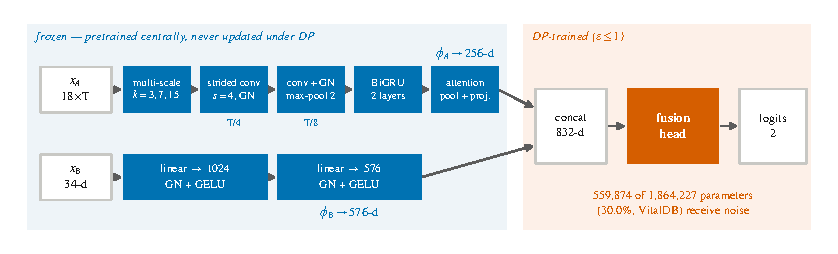
\includegraphics[width=\textwidth]{fig2_backbone.pdf}
\caption{Encoder--fusion backbone and the privacy boundary. Both encoders are
pretrained centrally and frozen; only the fusion head is trained under
differential privacy, so noise is applied to $559{,}874$ of $1{,}864{,}227$
parameters. Section~\ref{sec:method:backbone} defines the two pretraining
configurations, and Section~\ref{sec:exp:impl} records which produced which
result. No batch normalization appears anywhere, because it mixes statistics
across a batch and would make the per-patient gradient ill-defined.}
\label{fig:backbone}
\end{figure*}

Two properties of the backbone are required by the privacy mechanism. First,
its parameters remain frozen throughout federated training, so all trainable
and privatized capacity resides in the fusion head, which holds $559{,}874$ of
the $1{,}864{,}227$ parameters. The private optimization is therefore close to
a linear probe over fixed features. Second, every normalization layer is a
group or layer normalization; no batch normalization is used. Batch
normalization mixes statistics across the examples of a batch, so per-example,
and therefore per-patient, gradients would not be well defined, and the
privacy accounting would be invalid. The recurrent layer is likewise
implemented in a form compatible with per-sample gradients.

The pretraining corpus must satisfy an additional condition. If the encoders
are pretrained on data from the federated clients, they have been exposed to
the protected population without a guarantee, and the budget reported for the
head does not describe the system end to end. PP-HFM therefore distinguishes
two encoder configurations.

In the \emph{oracle} configuration, the encoders are pretrained on the pooled
training data of the federated clients. This configuration does \emph{not}
provide a valid end-to-end guarantee and is not proposed for deployment. It is
used to characterize the mechanism, because it isolates the attainable
performance of the head-only recipe from the origin of the representation. In
the \emph{disjoint} configuration, a set of individuals is reserved before
federated training, disjoint at the individual level from every client's
training, validation and test splits, and the encoders are pretrained only on
this set. Disjointness is verified explicitly. This configuration provides the
guarantee claimed in this paper, and its utility cost is measured.
Section~\ref{sec:exp:impl} specifies which configuration produced each result,
and Section~\ref{sec:results:objectives} reports the cost of moving between
them.

\subsection{Patient-Level Privacy Mechanism}
\label{sec:method:threat}
\label{sec:method:privacy}

A clinical system must provide a guarantee about individuals, whereas the
standard mechanism provides one about records. Differentially private
stochastic gradient descent bounds the influence of a training \emph{record}
by clipping its gradient to a fixed norm and adding noise to the aggregate
\cite{ref6}. When each record corresponds to a distinct person, the two
coincide. In a monitoring dataset, however, a record is a fixed-length window
and a single operation yields many windows, so removing one patient removes as
many records as that patient contributed. An $(\varepsilon,\delta)$-differentially
private mechanism is $(k\varepsilon,\,k e^{(k-1)\varepsilon}\delta)$-differentially
private for groups of size $k$ \cite{ref8}. Applied at the mean group size of
this cohort, this conversion turns a nominal $\varepsilon = 1$ into
$\varepsilon \approx 8$ with $\delta \approx 9 \times 10^{-2}$, which does not
support a clinical claim. The gap between the two units is illustrated in
Fig.~\ref{fig:sensitivity}.

Whether the two units differ depends on the deployment. When each client
corresponds to a single individual, as in a wearable installation where one
participant carries one device, client-level, user-level and individual-level
guarantees coincide. When a client holds records from many individuals, as an
institution holding many patients does, the units differ for every
participant. The mechanism below addresses the second case. The framework
applies to both, but only the second exhibits the gap, and the evaluation is
organized accordingly.

\begin{figure}[!t]
\centering
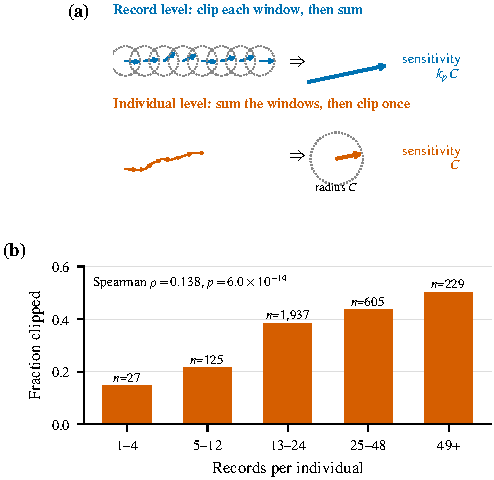
\includegraphics[width=\columnwidth]{fig02_privacy_unit.pdf}
\caption{Where the guarantee is decided. (a) Clipping each window to $C$ bounds
the influence of a \emph{window}: a patient contributing $k_p$ windows can
still displace the aggregate by $k_p C$. Summing a patient's windows before
clipping bounds the influence of the \emph{patient} at $C$, however many
windows that patient contributed. (b) On eICU at $C = 1$, the fraction of
individuals whose summed gradient is clipped rises with the number of records
they contribute; bar labels give individuals per bin.}
\label{fig:sensitivity}
\end{figure}

The mechanism enforces the guarantee at the point of clipping rather than by
conversion afterwards. The sampling unit is the patient: at each optimization
step, a client samples patients independently at a fixed rate, so the rate
entering the accountant is defined over patients rather than windows. For each
sampled patient, the gradients of all of that patient's windows are summed into
one per-patient gradient, and this sum is clipped to the clipping norm.
Clipping the sum makes the sensitivity patient-level: a patient can change the
aggregate by at most the clipping norm regardless of the number of windows,
whereas clipping each window separately would allow a change proportional to
that number. Gaussian noise calibrated to the same norm is then added once per
step to the aggregate of the clipped per-patient gradients, the result is
divided by the \emph{expected} batch size $q|\mathcal{P}_k|$, and the head
parameters are updated. The divisor must not be the realized batch size $|S|$:
the noise norm reveals the divisor, and $|S|$ depends on whether a given
patient is present, so normalizing by it releases information the accountant
does not cover. For the same reason a step whose sample is empty still
releases the noise. The mechanism is stated in
Algorithm~\ref{alg:patientdp}. For compute, at most $64$ records of a patient
enter its summed gradient; the rule is fixed and public, so the guarantee is
unaffected, and it truncates $4.1\,\%$ of eICU patients ($3.5\,\%$ of
training windows) and no VitalDB patient.

\paragraph{Objective solved} Without clipping, the expected step of client
$k$ is $|\mathcal{P}_k|^{-1}\sum_{p}g_p = \bar{k}_k\,\nabla F_k(\theta)$,
where $F_k$ is the record mean of the client's empirical risk and
$\bar{k}_k = n_k/|\mathcal{P}_k|$ the mean number of records per patient. A
local pass takes $|\mathcal{P}_k|/B$ such steps, $\bar{k}_k$ times fewer
than a record-level pass with $B$ records per step, so to first order in the
learning rate both displace client $k$ by $\eta\,(n_k/B)\,\nabla F_k$.
Before clipping, the patient-level mechanism therefore targets the declared
record-mean objective with unchanged client weights, in fewer and larger
steps. The argument is for the plain gradient step of
Algorithm~\ref{alg:patientdp}; the implementation passes the privatized
gradient to Adam, which is post-processing and leaves the guarantee unchanged
but rescales coordinates adaptively, so the argument holds only approximately.
Clipping is what changes the objective: each patient's summed gradient
is bounded as a whole, the surrogate of user-level DP-SGD \cite{ref11}, which
down-weights patients whose summed gradient exceeds $C$, typically those with
many records. This change belongs to the unit and is part of its measured
cost.

\begin{algorithm}[!t]
\caption{Patient-level private local update at client $k$}
\label{alg:patientdp}
\begin{algorithmic}[1]
\REQUIRE frozen $\theta_{\mathrm{enc}}$; head $\theta_{\mathrm{head}}$;
         patients $\mathcal{P}_k$ with records $\{W_p\}$; clip $C$;
         noise $\sigma$; rate $q$ from \eqref{eq:3}; step size $\eta$
\FOR{each local step}
  \STATE Sample $S \subseteq \mathcal{P}_k$, each $p$ independently w.p. $q$
  \FOR{$p \in S$}
    \STATE $g_p \leftarrow \sum_{(x,y)\in W_p}
            \nabla_{\theta_{\mathrm{head}}} \ell(f_\theta(x),y)$
            \hfill $\triangleright$ group by patient
    \STATE $\bar g_p \leftarrow g_p \cdot \min(1, C/\lVert g_p\rVert_2)$
            \hfill $\triangleright$ bound the sum
  \ENDFOR
  \STATE $\tilde g \leftarrow \frac{1}{q\,|\mathcal{P}_k|}\big(\sum_{p\in S}\bar g_p
          + \mathcal{N}(0,\sigma^2C^2I)\big)$
          \hfill $\triangleright$ also when $S=\emptyset$
  \STATE $\theta_{\mathrm{head}} \leftarrow \theta_{\mathrm{head}} - \eta\,\tilde g$
  \STATE Accountant.step($\sigma$, $q$)
\ENDFOR
\RETURN $\theta_{\mathrm{head}}$
\end{algorithmic}
\end{algorithm}

Accounting uses the same patient-level sampling rate, so the reported budget is
patient-level by construction. A single accountant instance persists for the
whole of a client's participation, so composition across rounds is preserved.
The construction has two costs, which this work measures: the number of
effective units per step decreases from windows to patients, and a patient with
many windows has their summed gradient clipped more strongly than a patient with
few. The dependence of this cost on the number of records per individual is
examined empirically by holding the first effect fixed and varying the second
(Section~\ref{sec:results:kscaling}).

\subsection{Noise Calibration Across Heterogeneous Clients}
\label{sec:method:calib}

The noise multiplier determines the budget for a given clipping norm, and
depends on the sampling rate and on the number of optimization steps of a
client. In a federated system partitioned by institution or specialty, these
quantities differ substantially between clients: a small client samples a
large fraction of its population per step, whereas a large client samples a
small one. A single noise multiplier calibrated for the most demanding client
satisfies the budget everywhere, but imposes that client's noise on every
other; on the external corpus, a hospital of fifteen patients sampled at rate
one sets the multiplier for all $187$ clients.

When each patient is held by exactly one client, as (A1) requires, the clients'
mechanisms act on disjoint sets of individuals, and by parallel composition the
guarantee for a patient is that of the client that holds them; individuals held
by several clients are treated where the scope of the theorem is stated. Each client therefore receives
its own noise multiplier $\sigma_k$, the smallest that meets the training
budget for that client's sampling rate and step count, Eq.~\eqref{eq:6}. The
multiplier depends only on the public client size, so it releases nothing
further. Accounting uses the privacy loss distribution accountant \cite{ref33},
which gives a tighter upper bound than R\'enyi accounting for the same
mechanism. The comparisons between arms in Section~\ref{sec:results:unit} use
the single most conservative multiplier, the maximum of $\sigma_k$, with
R\'enyi accounting, which holds every arm to the same noise.

Two details are essential. First, the number of optimization steps entering
the calibration must be the number the client actually executes; a count that
is too low underestimates the required noise. Second, the population and
sampling rate of each client are read from the partition files used in
training rather than from cached metadata, because metadata that no longer
matches the data produces a budget that is violated without any warning. Both
details are stated as part of the method because violations of either are not
detectable from training logs and can only be found by independent
recomputation.

\subsection{Two-Tier Hierarchical Aggregation}
\label{sec:method:agg}

In a flat federated system, every client update is sent to the cloud in every
round, so the wide-area link limits the update frequency. An intermediate
aggregation tier removes this limitation \cite{ref2, ref3}: several rounds of
local optimization and edge averaging are performed for each round of cloud
averaging, so the wide-area link is used once per group of local rounds.
PP-HFM adopts this organization, with $\tau_e$ edge rounds per cloud round, and
claims no novelty for the averaging rule.

Aggregation is performed in two stages, each weighted by the fixed number
of training records of the participants. The weights are public constants: a
weight computed from the records drawn in a given round would depend on which
patients were sampled and would reach the edge unprotected. Within a cloud round, each client
initializes from its edge model, performs one private local pass, and sends its
encoded update. The edge computes the weighted average over its clients and
returns it, and this is repeated $\tau_e$ times. The edges then report to the
cloud, which computes the weighted average over edges and broadcasts it as the
global model for the next round. Non-floating-point parameters are passed
through unchanged. The procedure is given in Algorithm~\ref{alg:round}.

\begin{algorithm}[!t]
\caption{PP-HFM cloud round $r$}
\label{alg:round}
\begin{algorithmic}[1]
\REQUIRE global model $\theta^{(r-1)}$; edge map $e(\cdot)$; edge rounds $\tau_e$
\STATE $\theta_e^{(r,0)} \leftarrow \theta^{(r-1)}$ for all edges $e$
\FOR{$s = 1$ \TO $\tau_e$}
  \FOR{each client $k$ \textbf{in parallel}}
    \STATE $\theta_k^{(r,s)} \leftarrow$ Algorithm~\ref{alg:patientdp}
           from $\theta_{e(k)}^{(r,s-1)}$
    \STATE Transmit $Q\big(\text{top-}\kappa(\theta_k^{(r,s)}-\theta_{e(k)}^{(r,s-1)})\big)$
  \ENDFOR
  \STATE Each edge aggregates by \eqref{eq:8}
\ENDFOR
\STATE Cloud aggregates by \eqref{eq:9} and broadcasts $\theta^{(r)}$
\RETURN $\theta^{(r)}$
\end{algorithmic}
\end{algorithm}

The parameter $\tau_e$ controls the trade-off of the hierarchy. With
$\tau_e = 1$, the edge tier is merged into the cloud tier, which recovers
conventional single-tier federated averaging; this configuration is used to
isolate the contribution of the hierarchy. Larger values reduce wide-area
transmissions proportionally but allow edge models to diverge further between
synchronizations. Because the privacy mechanism operates entirely within a
client and aggregation uses only privatized updates, $\tau_e$ affects
communication and convergence, and enters the guarantee only through the
number of optimization steps, which the calibration already accounts for.

\subsection{Update Encoding}
\label{sec:method:encoding}

A further component is adopted from established practice and is not claimed
as a contribution. It reduces the transmitted payload. Each
client update is sparsified by retaining only its largest-magnitude
coordinates, and the retained values are uniformly quantized to a reduced bit
width. The residual removed by sparsification is stored locally and added to
the next round's update, so suppressed coordinates are transmitted later rather
than lost. The encoding is applied after the privacy mechanism and is therefore
post-processing; by the post-processing property of differential privacy, it
does not affect the guarantee and can be tuned for bandwidth alone.

A private conformal threshold, released per client by the exponential
mechanism over ranks \cite{ref30, ref24} at $\varepsilon_{\mathrm{conf}} = 0.1$
with one score per calibration patient, was also evaluated. At about a hundred
calibration patients per client it does not attain coverage
(Section~\ref{sec:results}), so it is not part of the system, and the reported
budget is the training budget alone.

\subsection{Deployment Path and Inference Under a Latency Budget}
\label{sec:method:deploy}

The clinical value of the trained model depends on the delay between the
availability of a measurement and the return of a prediction, which is a
property of the deployment path. This path is therefore specified as part of
the system. The trained network is exported to a portable computation graph and executed
at full precision. Post-training eight-bit quantization \cite{ref26} was
evaluated as an alternative and rejected, because on a CPU provider it
increased rather than reduced latency (Section~\ref{sec:results}). Any
transformation of the released model after federated training is
post-processing and does not affect the privacy guarantee. Inference is executed at the edge tier rather
than in the cloud, so the wide-area link is not on the critical path.

The delay is decomposed into four separately measured stages, because an
end-to-end figure within budget may still be dominated by a removable stage.
Preprocessing constructs and normalizes the input tensors from the sensor
stream; the forward pass evaluates the exported graph; the threshold step of the evaluated conformal set, which is not deployed, is
kept as a conservative upper bound; and
a final stage converts the output into the format required by the consuming
system.

Latency is characterized by its distribution rather than its mean, and the
budget must be met at the 95th percentile, since a clinical service level is
defined by its tail. The measurement configuration is fixed in advance: the
full-precision graph is executed on a general-purpose CPU provider,
representing an edge node without an accelerator, for one thousand timed runs
after one hundred discarded warm-up runs, and each of the four stages is timed
within every run. A CPU provider is used because an edge deployment cannot be
assumed to have a GPU.

\subsection{Network and Energy Instrumentation}
\label{sec:method:instr}

Three of the four design objectives concern quantities that cannot be observed
from training: the wide-area traffic of the hierarchy, the reliability of update
delivery, and the energy consumed per round by each tier. These are properties
of the deployed topology and are therefore measured on simulated models of that
topology rather than estimated from parameter counts.

The network is modeled with the three tiers of Section~\ref{sec:method:arch}.
The device-to-edge segment uses a wireless local-area link and the
edge-to-cloud segment a point-to-point backhaul, so the asymmetry between
frequent local exchange over a low-cost link and infrequent global exchange
over a high-cost link is represented explicitly. Each round is simulated in
both directions, the downlink broadcast of the global model and the uplink
transmission of client updates. Traffic volume, delivery reliability and
end-to-end delay are recorded per round for the proposed configuration and for
the flat and centralized baselines. Per-round delay quantifies the latency
benefit of the hierarchy during training, which is distinct from the inference
latency of the deployment path in Section~\ref{sec:method:deploy}. Because the
payload is the compressed update of Eqs.~\eqref{eq:10}--\eqref{eq:11}, the
measured traffic is that of the specified system rather than of an
uncompressed approximation.

Energy is modeled per tier from the power characteristics of the hardware and
the completion time of the assigned work. The device tier represents
constrained embedded nodes, the edge tier server-class accelerated hardware,
and the cloud tier the aggregation host. Energy is reported per tier because a
hierarchical design redistributes work rather than reducing it, and an
aggregate figure would not show whether a saving at one tier is offset by an
increase at another.

The targets for these quantities were fixed in advance and are listed in
Table~\ref{tab:objectives}. The measured values are reported in
Section~\ref{sec:results}.

\begin{table}[!t]
\centering
\caption{Design objectives and their pre-registered targets. The problem
specification fixes a numeric threshold for communication reduction but asks
only that the latency benefit of the hierarchy be quantified, so O1b is stated
as a direction rather than a percentage. Measured values are reported in
Section~\ref{sec:results}.}
\label{tab:objectives}
\begin{tabular}{llc}
\toprule
& Quantity & Target \\
\midrule
O1  & Uplink traffic reduction vs.\ centralized & $\ge 50\%$ \\
O1b & Training-round latency vs.\ centralized   & improvement \\
O2a & Privacy budget, composed total            & $\varepsilon \le 1$ \\
O2b & Accuracy loss under the budget            & $\le 2$ pp \\
O3a & Inference latency, 95th percentile        & $< 100$ ms \\
O3b & Successful model updates                  & $> 99\%$ \\
O4  & Energy saving per round vs.\ centralized  & $\ge 20\%$ \\
\bottomrule
\end{tabular}
\end{table}

\subsection{Empirical Auditing of the Guarantee}
\label{sec:method:mia}

A differential privacy guarantee is an upper bound on the influence of an
individual. It does not show what an adversary achieves in practice, nor that a
system with a weaker guarantee is exploitable. Membership inference provides
this complementary measurement \cite{ref14}. PP-HFM is audited by
individual-level membership inference. Members are the patients in the
clients' training splits and non-members are patients held out entirely. Both
groups are scored by the same released model using the same procedure, so any
separation between them reflects membership.

Two attacks of different strength are used. The first compares each patient's
mean per-record loss with a global threshold \cite{ref15}. Aggregation to the
patient level before thresholding is essential: a per-record attack measures
record membership, which a record-level guarantee already protects, whereas
averaging over a patient's records converts weak per-record signals into a
per-individual signal. The second is a likelihood-ratio attack \cite{ref17}
adapted so that the unit of membership is the patient. Shadow models are
trained on independently sampled halves of the patient population, with all
records of a patient assigned together, and each shadow is trained with the
same recipe as the target model. For each patient, the distribution of a
logit-scaled confidence statistic is estimated separately over the shadows that
include and exclude that patient, and membership is scored by the ratio of the
two densities. A global threshold is confounded by per-patient difficulty, so
the attack strength it reports is a lower bound on leakage rather than an
estimate \cite{ref16}. Per-patient calibration removes this confound, as
illustrated in Fig.~\ref{fig:lira}.

\begin{figure}[!t]
\centering
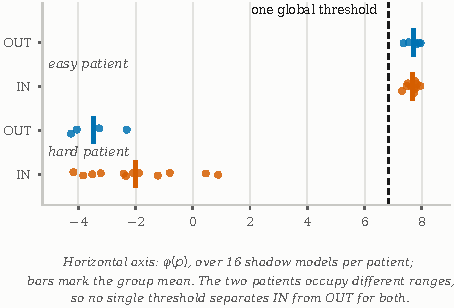
\includegraphics[width=\columnwidth]{fig4_lira.pdf}
\caption{Why per-patient calibration is necessary. Under a single global
threshold an easy non-member can outscore a hard member, so membership signal
is buried in per-patient difficulty. Fitting each patient's own in- and
out-distributions from shadow models removes that confound and scores
membership as a likelihood ratio.}
\label{fig:lira}
\end{figure}

Attacks are evaluated by the area under the receiver operating characteristic
curve and by the true-positive rate at low false-positive rates, because an
attack close to chance on average may still identify a few individuals with
high confidence. When the number of non-members is too small to resolve a
given false-positive rate, the value is reported as undefined rather than
interpolated.

A negative audit result is informative only if the attack is capable of
detecting leakage. The same procedure is therefore applied to a configuration
known to memorize, namely non-private training of the same head over the same
frozen encoders, and is required to detect clearly elevated leakage there. This
positive control is a precondition of the audit and is reported with every
result it qualifies.

% FLOAT NOTE: both algorithm floats are declared beside the text that cites
% them, not at the end of the section. Declared at the end — after the
% equations — LaTeX had no Methodology page top left and pushed Algorithm 2
% forward into Experimental Setup. A float never moves backwards; it must be
% declared where it can still be placed.
\subsection{Training Objective and Privacy Accounting}
\label{sec:method:objective}

Let $K$ clients be indexed by $k$, with client $k$ holding a local dataset
$\mathcal{D}_k$ of $n_k$ records and $n = \sum_k n_k$. Clients are assigned to
edges by a fixed map $e(\cdot)$. The records of client $k$ are partitioned by
individual into a set of patients $\mathcal{P}_k$, and $W_p$ denotes the
records contributed by patient $p$, with $k_p = |W_p|$; the partition is
constructed so that $W_p$ never spans two clients or two evaluation splits,
which holds by construction on eICU and on the person-level VitalDB partition
(Section~\ref{sec:experiments}).
Model parameters are written $\theta = (\theta_{\mathrm{enc}},
\theta_{\mathrm{head}})$, and $\ell$ is the cross-entropy; the loss is unweighted, because class
weights computed from the training labels would be a further unprotected
release. The
notation is summarized in Table~\ref{tab:notation}.

\begin{table}[!t]
\centering
\caption{Notation.}
\label{tab:notation}
\begin{tabular}{ll}
\toprule
Symbol & Meaning \\
\midrule
$K$, $E$              & number of clients, of edge aggregators \\
$\mathcal{P}_k$, $W_p$ & patients at client $k$; records of patient $p$ \\
$k_p = |W_p|$         & records contributed by patient $p$ \\
$R$, $\tau_e$         & cloud rounds; edge rounds per cloud round \\
$B$                   & patients sampled per optimization step \\
$C$, $\sigma$         & clipping norm; noise multiplier \\
$q$                   & Poisson sampling rate over patients \\
$(\varepsilon,\delta)$ & privacy budget \\
$\theta_{\mathrm{enc}}$, $\theta_{\mathrm{head}}$ & encoder, fusion-head parameters \\
\bottomrule
\end{tabular}
\end{table}

The learning objective is the standard weighted empirical risk over clients,
\begin{equation}
\begin{aligned}
\min_{\theta}\; F(\theta) &= \sum_{k=1}^{K} \frac{n_k}{n} F_k(\theta), \\
F_k(\theta) &= \frac{1}{n_k}\!\!\sum_{(x,y)\in\mathcal{D}_k}\!\!
               \ell\big(f_\theta(x), y\big),
\end{aligned}
\tag{1}
\label{eq:1}
\end{equation}
minimized only over $\theta_{\mathrm{head}}$, since $\theta_{\mathrm{enc}}$ is
pretrained on a disjoint public population and held fixed,
\begin{equation}
\theta_{\mathrm{enc}}\ \text{fixed},
\qquad
\theta_{\mathrm{head}} \leftarrow \text{privately optimized}.
\tag{2}
\label{eq:2}
\end{equation}

At each optimization step client $k$ draws a subset $S \subseteq \mathcal{P}_k$
by including each patient independently with probability
\begin{equation}
q_k = \min\!\Big(1,\ \frac{B}{|\mathcal{P}_k|}\Big),
\tag{3}
\label{eq:3}
\end{equation}
a rate defined over patients rather than records, which makes the accounted
quantity patient-level. For each sampled
patient the record gradients are accumulated and the sum is bounded,
\begin{equation}
\begin{aligned}
g_p &= \!\!\sum_{(x,y)\in W_p}\!\! \nabla_{\theta_{\mathrm{head}}}\,
       \ell\big(f_\theta(x), y\big), \\
\bar{g}_p &= g_p \cdot \min\!\left(1, \frac{C}{\lVert g_p \rVert_2}\right).
\end{aligned}
\tag{4}
\label{eq:4}
\end{equation}
Equation~\eqref{eq:4} determines the unit of the guarantee: because the bound
is applied to the sum, the influence of patient
$p$ is at most $C$ irrespective of $k_p$, whereas bounding each record
separately would admit an influence of $k_p C$. A single perturbation scaled to
the same norm is then applied to the aggregate,
\begin{equation}
\tilde{g} = \frac{1}{q_k |\mathcal{P}_k|}\left( \sum_{p \in S} \bar{g}_p
+ \mathcal{N}\!\big(0, \sigma^2 C^2 I\big) \right),
\tag{5}
\label{eq:5}
\end{equation}
where the divisor is a public constant rather than the realized $|S|$,
and the head is updated by $\theta_{\mathrm{head}} \leftarrow
\theta_{\mathrm{head}} - \eta\,\tilde{g}$.

Each client uses the smallest noise multiplier that meets the training budget
for its own sampling rate and step count,
\begin{equation}
\sigma_k = \min\big\{\sigma :\;
\varepsilon_k\big(\sigma,\, q_k,\, T_k\big)
\le \varepsilon\big\},
\tag{6}
\label{eq:6}
\end{equation}
where $\varepsilon_k$ is obtained from the privacy loss distribution accountant
\cite{ref33}, or from a R\'enyi accountant \cite{ref7, ref29} for the
single-multiplier arms $\sigma^{\star} = \max_k \sigma_k$, and the step count
is the number the client executes,
\begin{equation}
T_k = R\,\tau_e\,\max\!\Big(1, \Big\lfloor \frac{|\mathcal{P}_k|}{B} \Big\rfloor\Big)
\tag{7}
\label{eq:7}
\end{equation}
for the patient sampler of Algorithm~\ref{alg:patientdp}. $T_k$ must equal
the executed count; a count that differs from the executed one yields a budget
that is violated without any observable symptom.

Aggregation applies the weighted average at each tier. Writing
$\theta_k^{(r,s)}$ for the model of client $k$ after edge round $s$ of cloud
round $r$,
\begin{equation}
\theta_e^{(r,s)} = \!\!\sum_{k :\, e(k)=e}\!\!
\frac{n_k}{\sum_{j : e(j)=e} n_j}\; \theta_k^{(r,s)},
\tag{8}
\label{eq:8}
\end{equation}
\begin{equation}
\theta^{(r)} = \sum_{e=1}^{E} \frac{N_e}{\sum_{e'} N_{e'}}\;
\theta_e^{(r,\tau_e)},
\qquad
N_e = \!\!\sum_{k : e(k)=e}\!\! n_k .
\tag{9}
\label{eq:9}
\end{equation}

Updates are encoded before transmission. Sparsification retains the
$\kappa d$ largest-magnitude coordinates of an update $\Delta$ of dimension
$d$,
\begin{equation}
[\Delta^{\mathrm{sp}}]_i =
\begin{cases}
[\Delta]_i, & i \in \operatorname*{arg\,top}_{\kappa d} |\Delta| \\
0, & \text{otherwise,}
\end{cases}
\tag{10}
\label{eq:10}
\end{equation}
and the retained values are quantized uniformly to $b$ bits with step
$s = (v_{\max}-v_{\min})/(2^{b}-1)$,
\begin{equation}
Q(v) = v_{\min} + \operatorname{round}\!\Big(\frac{v - v_{\min}}{s}\Big)\, s .
\tag{11}
\label{eq:11}
\end{equation}
The residual $\Delta - \Delta^{\mathrm{sp}}$ is accumulated locally and added
to the next round's update. Both operations act on the already-perturbed
quantity of Eq.~\eqref{eq:5} and are therefore post-processing.


The guarantee is stated formally below. Two datasets are \emph{neighboring} if
one is obtained from the other by adding or removing every record of a single
patient. Three conditions are assumed. (A1) Each patient's records lie in the
training split of exactly one client, and the training, validation and test
cohorts are disjoint in patients. (A2) The following are public: the
architecture, the encoder parameters $\theta_{\mathrm{enc}}$, which are
pretrained on a patient-disjoint public pool, all hyperparameters
$(R,\tau_e,B,C,\sigma,\eta,\kappa,b)$, the edge map, the input standardization constants, and the declared client
sizes $|\mathcal{P}_k|$ and $n_k$, which are fixed before training; $q_k$,
$T_k$, $\sigma_k$ and the aggregation weights are computed from them and never
from the data.
(A3) The forward pass of a record depends on that record alone; the model
contains no normalization across records, such as batch normalization, so the
gradient of one patient's records is unaffected by any other patient.

\begin{theorem}[Patient-level guarantee]
\label{thm:guarantee}
Under (A1)--(A3), let each $\sigma_k$ satisfy Eq.~\eqref{eq:6}. The transcript of a
PP-HFM run, consisting of every encoded client update, every edge and cloud
model, and the model selected on the validation cohort, is
$(\varepsilon,\delta)$-differentially private with respect to
each training patient, under adding or removing all records of one patient
with the parameters of (A2) held fixed.
\end{theorem}

\begin{IEEEproof}
Fix a training patient $p$, held by client $k$ by (A1). \emph{One step.} Given
the model entering a step, the per-patient gradients $\bar g_{p'}$,
$p' \neq p$, are unchanged by the presence of $p$ by (A3), and
$\lVert \bar g_p \rVert_2 \le C$ by Eq.~\eqref{eq:4}. The noisy sum in
Eq.~\eqref{eq:5} is therefore a Poisson-subsampled Gaussian mechanism with rate
$q_k$, noise $\sigma C$ and $\ell_2$-sensitivity $C$ under addition or removal
of $p$, whose privacy loss is bounded in \cite{ref29, ref33}. Division by the
public constant $q_k|\mathcal{P}_k|$ and the optimizer update are
post-processing. \emph{Composition at client $k$.} Each step takes as input the
outputs of earlier steps, of other clients and public quantities, so the $T_k$
steps compose adaptively, and R\'enyi divergences add \cite{ref7}. The
accountant evaluates the composed bound exactly for $(\sigma,q_k,T_k)$, and
Eq.~\eqref{eq:6} ensures $\varepsilon_k \le \varepsilon$ at
$\delta$. Because $\sigma_k$ is a function of the public $|\mathcal{P}_k|$ and
$T_k$ only, using a different multiplier at each client releases nothing. \emph{Other clients.} By (A1) no other client accesses
the records of $p$; its outputs are randomized functions of its own data,
public quantities and messages already released, and therefore contribute no
privacy loss with respect to $p$. \emph{The hierarchy.} Sparsification with a
locally stored residual, quantization, edge and cloud averaging with the public
weights of Eqs.~\eqref{eq:8}--\eqref{eq:9}, and broadcast are functions of
released outputs and public quantities, and selection on the validation cohort
uses data disjoint from $p$ by (A1); all are post-processing.
\end{IEEEproof}

\begin{corollary}[Coincidence of the units]
\label{cor:k1}
If every patient contributes one record, Algorithm~\ref{alg:patientdp} is
differentially private stochastic gradient descent with Poisson sampling over
records at rate $q_k$, with the same clipping norm and noise. For equal
$(B, T_k, \sigma, C)$ the patient-level and record-level mechanisms are the
same mechanism, so a difference between them at one record per patient
measures seed variation or an implementation difference, not a property of the
privacy unit.
\end{corollary}

The theorem bounds what the guarantee reveals; the next statement predicts what
it costs. In the scaling experiments of Section~\ref{sec:results:kscaling},
$P$ individuals each contribute exactly $k$ records, so the record-level arm
minimizes $F(\theta) = \frac{1}{Pk}\sum_{p}\sum_{w \in W_p} \ell_w(\theta)$
and the individual-level arm minimizes the same $F$ written as
$\frac{1}{P}\sum_p \bar\ell_p(\theta)$, with
$\bar\ell_p = \frac{1}{k}\sum_{w\in W_p}\ell_w$.

\begin{proposition}[Cost in records per individual]
\label{prop:scaling}
Let each $\ell_w$ be convex and $L$-Lipschitz on a parameter domain of diameter
$D$ in $\mathbb{R}^d$, and let both arms be trained by differentially private
gradient descent at the same $(\varepsilon,\delta)$, and let
$\Lambda = LD\sqrt{d\log(1/\delta)}/\varepsilon$.
(i) The excess empirical risk of the record-level arm is at most
$c_{\mathrm{rec}}\Lambda/(Pk)$ and that of the individual-level arm at most
$c_{\mathrm{ind}}\Lambda/P$, with constants independent of $k$; both rates are
tight in the worst case up to logarithmic factors. (ii) If both arms attain their rate with a common
constant $c$, the gap is $A(1 - 1/k)$ with $A = c\Lambda/P$.
\end{proposition}

\begin{IEEEproof}
For $n$ units with convex $L$-Lipschitz losses, private gradient descent attains
excess empirical risk $O(LD\sqrt{d\log(1/\delta)}/(n\varepsilon))$, and this rate
is tight up to logarithmic factors \cite{ref31}. The record-level arm has $n = Pk$ units. In the
individual-level arm the unit is $\bar\ell_p$, which is $L$-Lipschitz as an
average of $L$-Lipschitz losses; clipping the summed gradient at $C$ equals
clipping the gradient of $\bar\ell_p$ at $C/k$, a rescaling that leaves the
guarantee unchanged, so the mechanism is private gradient descent over $n = P$
units. This gives (i), and (ii) follows by subtraction.
\end{IEEEproof}

Part (ii) rests on an assumption that (i) does not supply: upper bounds with
different constants do not determine the attained gap. The form $A(1-1/k)$ is
therefore a \emph{scaling hypothesis} that the proposition motivates, not a
theorem, and it is tested empirically, including out of sample. Moreover, the
proposition concerns bounds for convex losses, whereas the head is not convex
and the reported metric is average precision rather than excess risk. The
hypothesis therefore concerns the \emph{shape} of the cost, not its magnitude:
a gap of the form $A(1 - 1/k)$ with one free parameter, zero at $k = 1$, and an
individual-level arm whose utility does not depend on $k$. It also identifies
what would recover the cost. Additional records per individual reduce the
variance of $\bar\ell_p$'s gradient, but a clipping bound fixed around zero
cannot exploit this; mechanisms that clip around an estimate of the
per-individual mean can, and attain user-level rates that improve with $k$
\cite{ref32}. Rescaling the summed gradient by the record count, tested in
Section~\ref{sec:results:kscaling:nd}, is not such a mechanism.

The theorem fixes what is and is not covered. On eICU and on the
person-level VitalDB partition the unit is the person. On the case-level
VitalDB partition the unit is the surgical case: $230$ of $5{,}974$ people
($3.9\,\%$) underwent more than one operation, and for them the guarantee
holds per operation and extends to the person only by group privacy over at
most $14$ cases, composed across clients for the $68$ training persons whose
cases lie on two. On eICU, where clients are hospitals, the stays of $2{,}177$ of $74{,}327$ training persons ($2.9\,\%$) lie at two to four hospitals, so in the source partition (A1) fails for them. The privacy-cost and end-to-end runs therefore use a partition in which each such person is moved, with all their records, to the hospital holding most of their stays ($49{,}939$ training records; likewise $509$ validation and $589$ test persons); no record is excluded and every split is unchanged. In that partition every training and validation person is held by one hospital, so (A1) holds and the guarantee is $\varepsilon_{\mathrm{train}} = 0.9$ for every training person, verified independently for every client of every run (privacy-loss-distribution bounds $[0.880, 0.900]$; R\'enyi accountant $0.974$), and the evaluated conformal release adds $\varepsilon_{\mathrm{conf}} = 0.1$ once per person. The remaining eICU analyses (system objectives other than O2, scaling grid, clipping rule and prior systems) use the source partition, in which the per-client budget composes across the hospitals that hold a person: with the headline accountant, at most $1.32$, $1.64$ and $1.92$ for the $2{,}097$, $75$ and $5$ persons at two, three and four hospitals (R\'enyi: $1.42$, $1.77$, $2.08$), and at most $m\varepsilon$ in general; arms compared with each other share the partition. On the wearable deployment each client is one participant, and the
mechanism evaluated there is record-level; a person-level guarantee would
require client-level privacy at the edge, which is not evaluated. Outside the
guarantee are the validation cohort, which is used without noise for checkpoint
selection, the input standardization constants, which are computed once from
the training cohort, and the declared client sizes, which are treated as
public, as is conventional for privately trained models \cite{ref6}. Adding or
removing a patient changes the realized cohort but not the mechanism, because
every parameter is fixed by the declared sizes before training; this is the
setting in which the Poisson-subsampled Gaussian is analyzed
\cite{ref29, ref33}. In the experiments the declared sizes equal the realized
cohort sizes; where a size is sensitive, it can be replaced by a coarse public
value or released by a private count, and the theorem holds for whichever
declared values are used. Table~\ref{tab:scope} lists, for each evaluated configuration, the unit,
the provenance of the encoders and standardization constants, the accounting
and what the guarantee covers. The implementation of the accounting is
additionally checked by a suite of 17 regression checks, seven of which cover
it: composition of the budget across calls, release and accounting of noise at
every step with the expected-batch divisor, one conformal score per calibration
patient, and per-client multipliers within the budget. These are
implementation-level checks of the accounting configuration; they do not by
themselves establish the guarantee.

\begin{table*}[!t]
\centering
\caption{Scope of the guarantee in each evaluated configuration}
\label{tab:scope}
\footnotesize
\setlength{\tabcolsep}{4pt}
\begin{tabular}{>{\raggedright\arraybackslash}p{4.8cm}>{\raggedright\arraybackslash}p{2.3cm}>{\raggedright\arraybackslash}p{3.6cm}>{\raggedright\arraybackslash}p{3.3cm}>{\raggedright\arraybackslash}p{2.7cm}}
\toprule
Configuration & Unit & Encoders / standardization & Accounting & Guarantee covers \\
\midrule
eICU, headline (one hospital per person) & patient & disjoint / training cohort & $\sigma_k$, PLD; $0.9 + 0.1$ & training transcript \\
eICU, pool-fitted constants (one hospital per person) & patient & disjoint / public pool & $\sigma_k$, PLD; $0.9 + 0.1$ & end to end \\
VitalDB, person-level headline & person & oracle / training cohort & $\sigma_k$, PLD; $0.9 + 0.1$ & transcript; (A2) violated \\
VitalDB, disjoint encoders (case-level) & surgical case & disjoint / training cohort & $\sigma_k$, PLD; $0.9 + 0.1$ & transcript, per case \\
VitalDB, cost of the unit and audit (person-level) & person vs record & oracle / training cohort & $\sigma_{\max}$, RDP; $1.0 + 0.5$ & training transcript \\
Scaling grids, clipping rule (VitalDB case-level; eICU) & individual vs record & oracle (VitalDB), disjoint (eICU) / training & $\sigma_{\max}$, RDP; $0.8$--$1.0 + 0.2$--$0.5$ & training transcript$^{\ddagger}$ \\
eICU, prior systems (source partition) & patient & disjoint / training cohort & $\sigma_k$, PLD; $0.9 + 0.1$ & training transcript$^{\ddagger}$ \\
WEAR & record (= participant) & oracle / training cohort & record-level; $0.766 + 0.2$ & transcript, per record \\
\bottomrule
\end{tabular}
\par\vspace{3pt}\parbox{\linewidth}{\footnotesize Unit: neighboring datasets differ by all records of one patient, person or case, or by one record; ``vs'' marks a comparison of two arms. Accounting: $\varepsilon_{\mathrm{train}} + \varepsilon_{\mathrm{conf}}$ at $\delta = 10^{-5}$; $\sigma_k$, per-client multipliers; $\sigma_{\max}$, one worst-client multiplier; PLD, privacy-loss-distribution accountant; RDP, R\'enyi accountant. The conformal release was evaluated and is not part of the deployed system. Arms compared with each other share one configuration. Other analyses (recipe, ablation, fusion, attribution) are labeled with their partition and mechanism in Section~\ref{sec:results}. $^{\ddagger}$eICU on the source partition: for the $97.1\,\%$ of training persons at one hospital; the $2.9\,\%$ at two to four hospitals compose the mechanisms of those hospitals ($\varepsilon_{\mathrm{train}} \le 1.32$--$1.92$ with $\sigma_k$ and PLD).}
\end{table*}

Finally, the audit statistic of Section~\ref{sec:method:mia} is the
logit-scaled confidence of a patient, averaged over that patient's records,
\begin{equation}
\varphi(p) = \frac{1}{|W_p|}\sum_{(x,y)\in W_p}
\Big( z_y(x) - \log\!\!\sum_{j \neq y} e^{z_j(x)} \Big),
\tag{12}
\label{eq:14}
\end{equation}
which is the numerically stable form of $\log\!\big(\hat{p}_y/(1-\hat{p}_y)\big)$,
and membership is scored by the ratio of the fitted in- and out-densities,
\begin{equation}
\Lambda(p) = \log
\frac{\mathcal{N}\!\big(\varphi(p);\, \mu_{\mathrm{in}}(p), \sigma^2_{\mathrm{in}}(p)\big)}
     {\mathcal{N}\!\big(\varphi(p);\, \mu_{\mathrm{out}}(p), \sigma^2_{\mathrm{out}}(p)\big)} .
\tag{13}
\label{eq:15}
\end{equation}



The objective in Eq.~\eqref{eq:1} is minimized over the fusion head only,
using the mechanism of Eqs.~\eqref{eq:3}--\eqref{eq:5} with the noise scale
given by Eq.~\eqref{eq:6}, while the encoders remain frozen. Optimization uses
stochastic gradient descent on the perturbed gradient. The reported model is
selected by validation performance.

%==============================================================================
% experiments.tex — Experimental Setup for PP-HFM
% Self-contained \section{}; \input this into main.tex (never compile alone).
%
% Structured after the house experimental-setup template: Datasets,
% Implementation Details, Evaluation Metrics (defined as numbered equations),
% Experimental Protocol, closing with a forward pointer to Results.
%
% Equation numbering CONTINUES from method.tex, which ends at (15).
%
% Every figure here is established fact verified against an artifact:
%   partition_meta.json   client counts, edge map, split sizes, class balance
%   datasets.py registry  channel counts, modality contracts, pairing
%   labels.npy            outcome prevalence
%   installed packages    library versions
% No measured outcome appears in this section; outcomes are in Section V.
% READABILITY PASS 2026-10-21: formal register; equations/figure verbatim.
%==============================================================================

\section{Experimental Setup}
\label{sec:experiments}

Fig.~\ref{fig:workflow} outlines the study from partitioning to audit.

\begin{figure*}[!t]
\centering
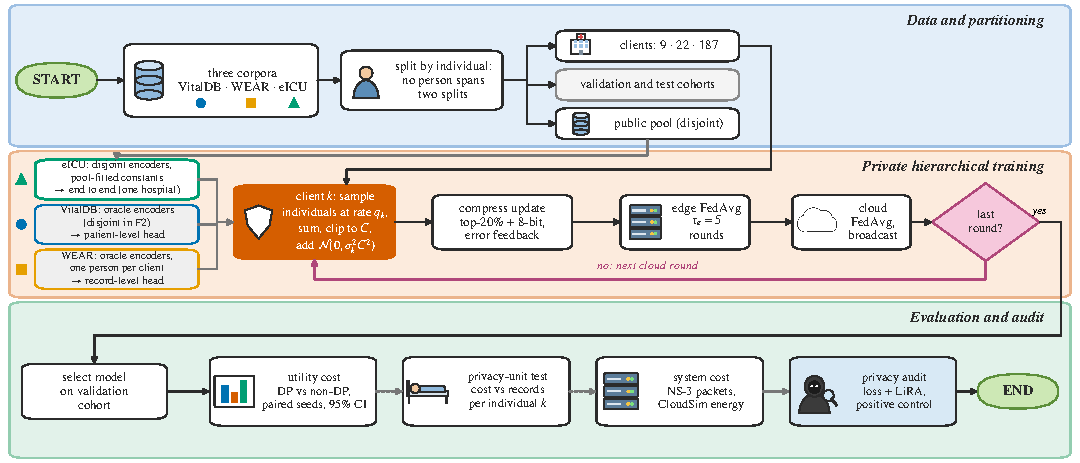
\includegraphics[width=\textwidth]{fig00_workflow.pdf}
\caption{Study workflow: individual-level partitioning, per-corpus encoder
configuration (end to end on eICU only, for individuals at one hospital), private hierarchical training and
paired evaluation with an attack audit.}
\label{fig:workflow}
\end{figure*}

\subsection{Datasets}

The framework is evaluated on two publicly available multimodal corpora:
VitalDB \cite{ref20}, a clinical monitoring collection of non-cardiac surgical
cases, and WEAR \cite{ref21}, an outdoor activity collection combining
body-worn inertial sensing with egocentric video. A third corpus, the eICU
Collaborative Research Database \cite{ref27}, distributed through PhysioNet
\cite{ref28} under a credentialed data-use agreement, serves as an external
clinical corpus. In all three corpora, the two modalities originate from the
same individual and are paired at the source rather than by a construction
rule. This
property is necessary for a claim about fusion, since a fusion benefit under
rule-based pairing may reflect the rule rather than complementary information.
The corpora also cover the two deployment regimes relevant to the privacy
mechanism: a client holding many individuals and a client holding one.

In VitalDB, modality~A is the intraoperative monitoring record with eighteen
channels, namely nine numeric physiological trends and nine binary indicators
of whether each trend was recorded. Modality~B is a thirty-four-dimensional
vector of preoperative clinical and laboratory variables. All channels of a
case originate from the same patient during the same operation and are
time-aligned at capture across the waveform digitizer, the patient monitor and
the anesthesia machine. The prediction target is postoperative admission to
intensive care, which is positive in $18.84\,\%$ of windows ($19.65\,\%$ in
the case-level partition defined below). In WEAR,
modality~A consists of twelve inertial channels and modality~B is a
$2048$-dimensional two-stream video feature computed over the same interval and
synchronized in hardware. The task is activity recognition over eighteen
classes.

In eICU, modality~A consists of twelve channels: six vital signs recorded
during the ICU stay (heart rate, respiratory rate, oxygen saturation, systolic
and diastolic arterial pressure, and temperature) and six binary indicators of
whether each was observed. The first $24$ hours after unit admission are
divided into non-overlapping $60$-minute windows of twelve $5$-minute slots,
and a window is retained only if at least three slots are observed.
Modality~B is a five-dimensional vector recorded at or before admission (age,
sex, admission weight, admission height and the APACHE score) for the same
stay. The prediction target is in-unit mortality, with a prevalence of
$0.0422$. Individuals who die within the observation window are excluded,
since their final windows are peri-mortem and pose no prediction problem.
Prediction is therefore made at hour $24$, when the APACHE score, computed
from the worst values of the first day, is available. The
resulting corpus contains $3{,}782{,}805$ windows from $185{,}140$ stays of
$132{,}736$ individuals.

Each corpus is partitioned into disjoint training, validation and test
subsets, which are fixed across all experiments, so no record appears in more
than one subset and all arms use the same split. VitalDB is evaluated on two
partitions, both distributing cases across nine clients by surgical specialty
and two edge aggregators. The \emph{person-level} partition assigns each
person to one split and one client; cases that would place a person in a
second split or on a second client are removed ($200$ cases). It contains
$33{,}491$ training, $6{,}773$ validation and $6{,}895$ test windows from
$4{,}221$, $868$ and $885$ persons, with $7.9$ training windows per
individual on average. The \emph{case-level} partition of the earlier
experiments splits by operation ($34{,}044$, $7{,}308$ and $7{,}360$ windows
from $6{,}257$ operations); in it, $55$ of $940$ test persons also have a
training case and $68$ training persons span two clients, so its results
protect the operation rather than the person. The privacy cost, the cost of
the unit and the comparison with prior systems are person-level; all other
VitalDB results are case-level and marked as such. No test case of either
partition was used to pretrain the encoders. For WEAR, the partition contains $26{,}424$ training,
$5{,}395$ validation and $5{,}969$ test windows across twenty-two clients, one
per participant, also assigned to two edges. Partitioning by specialty rather
than at random produces realistic heterogeneity, since specialties differ in
case mix, outcome prevalence and routinely recorded channels
(Fig.~\ref{fig:noniid}). For eICU, the clients are the hospitals themselves,
taken as given rather than constructed. Of $206$ hospitals, those with fewer
than $200$ windows or with no positive outcome are pooled into a single
client, giving $187$ clients assigned to two edge aggregators, with a median of
$444$ individuals per client and $28.50$ records per individual. Splits are
made by individual, stratified by outcome within each client, because an
individual may be admitted more than once, and a stay-level split would place
the same person in both training and test data. Case-level metrics on eICU are
grouped by stay rather than by individual, because the outcome of a person can
differ between admissions. The validation subset is used only for model
selection, and the test subset only for final evaluation.

\begin{figure*}[!t]
\centering
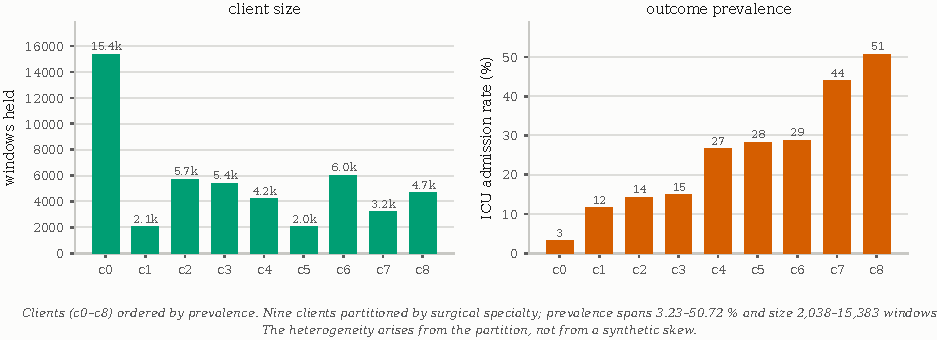
\includegraphics[width=\textwidth]{fig6_noniid.pdf}
\caption{Heterogeneity of the clinical partition (case-level). Partitioning by surgical
specialty rather than at random yields clients that differ by a factor of
seven in size and by more than fifteen in outcome prevalence, from $3.23\,\%$
to $50.72\,\%$. The skew is a property of how care is organized, not an
artifact imposed for the experiment.}
\label{fig:noniid}
\end{figure*}

Four controls are applied in preparing the clinical corpus, each preventing an
inflation of the reported results that would not be visible during training.
First, data are split by case, so all windows of an operation fall in the same
subset; a window-level split would place highly correlated near-duplicates of
training examples in the test set. Second, modality~B is restricted to
preoperative variables, and all intraoperative columns are excluded, because
interventions such as transfusion or vasopressor administration are given in
response to deterioration and therefore encode the outcome. Third, missing
values are not simply imputed: gaps are filled within a case and paired with
an explicit binary indicator, because, for example, an arterial line is placed
only in patients judged to be at risk, so its absence carries information
about acuity. Fourth, normalization statistics are computed over training cases
only, with estimators that handle missing values, because a naive estimator
returns an undefined statistic for a fully missing channel and propagates it to
every window. In addition, a separate set of individuals, disjoint at the
individual level from all client data, is reserved before federated training
and used only to pretrain the encoders, so that the reported budget holds end
to end. For eICU, this pool contains $526{,}867$ windows, leaving
$2{,}122{,}350$ training, $563{,}948$ validation and $569{,}640$ test windows
for the clients.

\subsection{Implementation Details}
\label{sec:exp:impl}

All arms use the same training configuration, so that differences can be
attributed to the mechanism under test. Each client performs one local pass per
federated call, five edge rounds are executed per cloud round, and training
runs for ten cloud rounds. The privatized gradient is passed to Adam
(learning rate $10^{-3}$, weight decay $10^{-4}$), which is post-processing,
with a per-individual clipping norm of one, $64$
individuals sampled per step in expectation, and a noise multiplier per client
from the calibration of \eqref{eq:6}.
Updates are sparsified to the largest twenty percent of coordinates and
quantized to eight bits before transmission, with error feedback of the
residual. The full budget goes to training: $\varepsilon = 0.9$ on the
clinical deployments. The encoders are pretrained centrally and then frozen, so the
privatized parameters are those of the fusion head only: $559{,}874$ of
$1{,}864{,}227$ parameters, or $30.0\,\%$.

Unless stated otherwise, all results, including the system-level objectives,
the privacy--utility comparisons and the membership-inference audit, were
obtained with the \emph{oracle} encoder configuration of
Section~\ref{sec:method:backbone}, in which the encoders were pretrained on the
pooled client training data. This configuration does not provide a valid
end-to-end guarantee. It is used because it isolates the behavior of the
privatized head from the origin of the representation, and because using the
same encoders in every arm keeps the comparisons between arms controlled. The
\emph{disjoint} configuration, which provides the guarantee, is evaluated
separately, and the difference is reported in
Section~\ref{sec:results:objectives} as the cost of a valid guarantee. On eICU,
every experiment that uses pretrained encoders uses the disjoint
configuration.
Absolute utilities should therefore be read as upper bounds for the deployable
configuration, whereas differences between arms, on which the claims rely, are
unaffected. All normalization layers are group or layer normalizations, as
explained in Section~\ref{sec:method:backbone}.

Models are implemented in PyTorch~2.5, with per-sample gradients and R\'enyi
accounting provided by Opacus~1.5. Deployment models are exported to ONNX at
full precision, and inference is timed with ONNX Runtime on the CPU
provider of a workstation (Intel Core i7-14700), since an edge node cannot be
assumed to have an accelerator; no edge hardware was used. Network behavior is simulated in ns-3~3.46,
with the device-to-edge segment over a wireless local-area link and the
edge-to-cloud segment over a point-to-point backhaul. Energy is modeled in
CloudSim~Plus separately for the device, edge and cloud tiers. Training was
performed on a single workstation with one NVIDIA RTX~A2000 GPU.
Table~\ref{tab:params} collects these parameters.

\begin{table}[!t]
\centering
\caption{Training and evaluation parameters}
\label{tab:params}
\footnotesize
\setlength{\tabcolsep}{4pt}
\begin{tabular}{@{}p{0.40\columnwidth}p{0.56\columnwidth}@{}}
\toprule
Parameter & Value \\
\midrule
Cloud rounds $R$; edge rounds $\tau_e$ & $10$; $5$ \\
Edge aggregators $E$ & $2$ (eICU scaling test: $2$--$16$) \\
Local passes per edge round & $1$ \\
Optimizer & Adam \\
Learning rate; weight decay & $10^{-3}$; $10^{-4}$ \\
Expected individuals per step $B$ & $64$ \\
Clipping norm $C$ & $1$ \\
Training budget & $\varepsilon = 0.9$, $\delta = 10^{-5}$ \\
Accountant & privacy loss distribution, per-client $\sigma_k$ \\
Records per patient (cap) & $64$ \\
Update encoding & top-$20\,\%$, $8$-bit, error feedback \\
Seeds & $5$ (paired); $3$ for grids \\
LiRA shadow models & $16$ \\
Latency timing & P95, $1{,}000$ runs, $100$ warm-up \\
Software & PyTorch~2.5, Opacus~1.5, ONNX Runtime, ns-3~3.46, CloudSim~Plus~8.5 \\
Hardware & one NVIDIA RTX~A2000 GPU \\
\bottomrule
\end{tabular}
\end{table}

\subsection{Evaluation Metrics}

Classification performance is assessed with two complementary measures. The
area under the receiver operating characteristic curve summarizes ranking
performance across all decision thresholds. Average precision summarizes the
precision--recall trade-off,
%
\begin{equation}
\mathrm{AP} = \sum_{n} \big(R_n - R_{n-1}\big)\, P_n,
\tag{14}
\label{eq:16}
\end{equation}
%
where $P_n$ and $R_n$ are the precision and recall at the $n$th threshold.
Average precision is reported because the clinical task is imbalanced, with
$18.84\,\%$ positive windows. Under this imbalance, accuracy is nearly
uninformative, since a constant negative prediction achieves about four-fifths
accuracy, and the area under the ROC curve is optimistic. Average precision
reflects performance on the minority class.

Metrics are also aggregated per individual. The model scores windows, but the
clinical question concerns an operation, and windows of the same case are
highly correlated, so window-level metrics overstate the effective sample size.
The predictions of a case are therefore averaged,
%
\begin{equation}
\bar{p}_c = \frac{1}{|W_c|} \sum_{w \in W_c} p_w ,
\tag{15}
\label{eq:17}
\end{equation}
%
giving one prediction per individual. Case-level metrics are computed from
$\bar{p}_c$ using the same expressions as for $p_w$.

Comparisons between arms are paired by seed, since the arms share their
partition, initialization schedule and calibration data. For $S$ paired seeds
with per-seed difference $d_s$, the reported interval is
%
\begin{equation}
\bar{d} \pm t_{S-1,\,0.975}\, \frac{s_d}{\sqrt{S}},
\tag{16}
\label{eq:18}
\end{equation}
%
where $s_d$ is the sample standard deviation of the differences. Student's $t$
distribution is used instead of a normal approximation because the number of
seeds is small. Seed counts are fixed before each comparison and are not
increased after inspecting the results.

Communication, latency, reliability and energy are reported as defined in
Section~\ref{sec:method:instr}, and every network quantity is measured on
rounds in which the payload traversed the simulated topology.

\subsection{Experimental Protocol}

The proposed system is compared with differentially private federated
averaging in three configurations, each isolating one design decision. The
first trains the full parameter vector under the privacy budget, which is the
conventional application of DP-SGD to a federated model. The second restricts
private optimization to the fusion head over randomly initialized frozen
encoders, isolating the effect of reducing the privatized dimension. The third
restricts private optimization to the fusion head over \emph{pretrained} frozen
encoders. This arm controls for a confound: without it, the benefit of
parameter-efficient private training cannot be separated from the benefit of
the pretrained representation. A non-private model trained with an otherwise
identical recipe provides the reference for the accuracy cost of the budget.
All arms share the partition, schedule, compression settings and evaluation
procedure, and differ only in the factor under test.

The same evaluation protocol is applied to every arm. The checkpoint with the
highest validation performance is retained, without use of test data. Each
retained checkpoint is evaluated once on the test subset, and all metrics are
computed from the same predictions with the same aggregation.

The privacy guarantee is audited by individual-level membership inference
using the two attacks of Section~\ref{sec:method:mia}. Each attack is also
applied to a configuration known to memorize, namely non-private training of
the same head over the same frozen encoders, as a positive control. A negative
result is accepted only if the same procedure detects clearly elevated leakage
on the control.

A further experiment separates the two sources of the cost of the
individual-level unit. Moving the guarantee from the record to the individual
both reduces the number of units sampled per step and bounds the summed
contribution of each individual, and the aggregate comparison cannot separate
the two. The number of units sampled per step is therefore held equal in both
arms, which removes the first effect and leaves only the clipping geometry,
and the number of training records retained per patient, $k$, is varied over
$\{1, 2, 4, 8\}$ with three seeds at $\varepsilon = 1$. Subsampling is applied
to the training partition only; validation and test sets are unchanged, so
every configuration is evaluated on the same held-out data. Because reducing
$k$ also reduces the training set size, absolute utility decreases with $k$ and
is not comparable across $k$. The quantity of interest is the paired difference
between arms at each $k$, where both arms use the same data, partition and
seed. At $k = 1$, a patient contributes a single record, so the two arms must
agree, which provides a falsification test of the design.

%==============================================================================
% results.tex — Results for PP-HFM
% Self-contained \section{}; \input this into main.tex (never compile alone).
%
% STATUS: partial. Only subsections whose experiments are COMPLETE and whose
% numbers are read from a results artifact appear here. Pending subsections are
% listed at the end of this file as comments, each naming the experiment and
% the artifact that will supply it. Do not write a number into this file that
% does not appear in a file under SIMULATORS/results/.
%
% Every figure quoted below is traceable:
%   objectives_vitaldb.json   O1, O1b, O2a, O2b, O3a, O3b, O4
%   objectives_wear.json      same, wearable deployment
%   latency_*.json            per-stage latency decomposition
%   ns3_results_*.csv         round latency, reliability (all rows packet-level)
%   cloudsim_results_*.csv    per-tier energy
%==============================================================================

\section{Results}
\label{sec:results}

\subsection{System-Level Objectives}
\label{sec:results:objectives}

The framework is evaluated on two deployments that differ in client
composition. In the clinical deployment, nine institutional clients hold the
records of $6{,}257$ patients, so each client contains many individuals, and
each individual contributes $7.8$ records on average. In the wearable
deployment, each of the twenty-two clients corresponds to a single participant
who contributes approximately $1{,}750$ records. The second deployment also
tests whether the system-level behavior generalizes across topology and payload
size.

Table~\ref{tab:results_objectives} reports the measured value of each design
objective of Table~\ref{tab:objectives}. All targets are met on the clinical
deployment. On the wearable deployment, all targets are met except the accuracy
bound, which is inconclusive.

\begin{table}[!t]
\centering
\caption{Measured outcomes against the pre-registered targets of
Table~\ref{tab:objectives}. Network quantities are measured at packet level on
every simulated round of both deployments. The accuracy row is a paired
comparison against a non-private reference trained under the identical recipe;
$^{\dagger}$ marks an interval that spans its threshold and is therefore
inconclusive at the pre-registered sample size.}
\label{tab:results_objectives}
\small
\setlength{\tabcolsep}{4pt}
\begin{tabular}{llrrl}
\toprule
& Quantity & Clinical & Wearable & Target \\
\midrule
O1  & Uplink reduction   & $90.8\%$   & $96.1\%$   & $\ge 50\%$ \\
O1b & Round latency      & $16.9\%$   & $21.7\%$   & improvement \\
O2a & Budget (composed)  & $0.970$    & $0.966$    & $\varepsilon \le 1$ \\
O2b & Accuracy change    & $-0.92$ pp & $1.97^{\dagger}$ pp & $\le 2$ pp \\
O3a & Latency (P95)      & $4.58$ ms  & $1.22$ ms  & $< 100$ ms \\
O3b & Update success     & $100.00\%$ & $99.94\%$  & $> 99\%$ \\
O4  & Energy saving      & $72.3\%$   & $76.8\%$   & $\ge 20\%$ \\
\bottomrule
\end{tabular}
\end{table}

\begin{table}[!t]
\centering
% !! STALE: latency_vitaldb.json (2026-09-06) gives total mean 2.912 / P95 3.048 ms
% !! on the FP32 graph, 200 runs. Values and caption below are from an older run.
% !! Resolve before submission (see session notes 2026-10-21).
\caption{Inference latency decomposition, integer-quantized graph on a CPU
provider, 1000 timed executions after 100 discarded warm-up executions.}
\label{tab:latency}
\begin{tabular}{lrr}
\toprule
Stage & Mean (ms) & P95 (ms) \\
\midrule
Preprocessing              & 0.140 & 0.147 \\
Forward pass               & 4.221 & 4.395 \\
Conformal set construction & 0.030 & 0.037 \\
Post-processing            & 0.011 & 0.014 \\
\midrule
Total                      & 4.401 & 4.582 \\
\bottomrule
\end{tabular}
\end{table}

\begin{figure*}[!t]
\centering
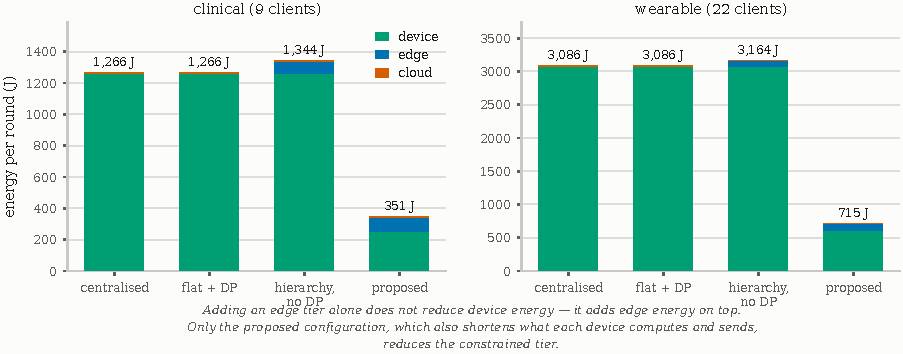
\includegraphics[width=\textwidth]{fig7_energy.pdf}
\caption{Energy per training round, attributed by tier, on both deployments.
The hierarchy alone redistributes work without reducing it: device energy is
unchanged and edge energy is added. Only the proposed configuration reduces the
energy of the constrained tier.}
\label{fig:energy}
\end{figure*}

All network quantities are measured on every simulated round. An earlier
simulator configuration evaluated one round in ten at packet level and composed
the remaining rounds analytically. The two approaches disagree: the analytical
model placed the communication term of the centralized baseline at $256$ ms,
whereas the simulated network delivers $23.6$ ms, which overstated the latency
benefit of the hierarchy by a factor of about four. No analytically composed
rounds contribute to the values reported here.

The reported privacy budget is the composed total. Training accounts for
$\varepsilon = 0.7705$ and the release of the conformal calibration quantile
for a further $0.2000$, giving $0.970$ against a budget of one. Reporting only
the training term would understate the expenditure by $23\,\%$.

\subsubsection{Communication and latency}
Two-tier aggregation reduces uplink traffic by $90.8\,\%$ relative to
centralized training, against a target of $50\,\%$. The measurement is taken
from the deployed compressor and includes the index array that top-$\kappa$
sparsification transmits with the retained values, which analytical payload
estimates omit and which is not negligible at high sparsity.

The hierarchy also reduces the end-to-end latency of a training round from
$90.5$ ms to $75.2$ ms in the clinical deployment, a reduction of $16.9\,\%$.
The reduction is positive in every simulated round, ranging from $8.2\,\%$ to
$25.8\,\%$. It is smaller than the traffic reduction because the communication
term falls from $23.6$ ms to $16.5$ ms, while the compute terms (sensing,
preprocessing, inference and aggregation) are common to all topologies and
dominate the total. The hierarchy reduces link time, not computation.

In the wearable deployment, round latency falls from $104.5$ ms to $81.8$ ms,
or $21.7\,\%$, with the communication term falling from $37.6$ ms to
$23.2$ ms. The larger reduction is consistent with the larger topology:
twenty-two stations contend for the same wireless medium rather than nine, so
uplink latency is a larger share of the total. The latency benefit of the
hierarchy therefore depends on the topology.

\subsubsection{Cost of a valid guarantee}
The results above were obtained with the oracle encoder configuration, in which
the frozen representation was pretrained on the pooled client training data.
This configuration does not provide a valid end-to-end guarantee, and its
utility is therefore an upper bound. With the disjoint configuration, in which
the encoders are pretrained only on a population reserved before federated
training and disjoint from every client, the area under the ROC curve decreases
by $0.0322$ $(0.8429 \rightarrow 0.8107)$, by $0.0310$ at the case level, and
average precision by $0.0763$. This difference is the cost of an end-to-end
valid guarantee. Comparisons between arms are unaffected, because all arms
share the same encoders.

\subsubsection{Privacy and utility}
The composed budget of $0.970$ satisfies the requirement $\varepsilon \le 1$.
Relative to a non-private reference trained with the same recipe, the change in
balanced accuracy is $-0.92$ pp, with a paired $95\,\%$ confidence interval of
$[-2.82, +0.99]$ over five seeds. The interval contains zero, so no accuracy
cost is detectable at this sample size. The requirement of at most $2$ pp is
met.

On the wearable deployment, the same comparison gives $1.967$ pp with an
interval of $[1.760, 2.173]$ over fifteen seeds. The interval spans the $2$ pp
threshold, so this objective is \emph{inconclusive}. The seed count was fixed
in advance and was not increased after inspecting the interval.

\subsubsection{Quality of service}
Table~\ref{tab:latency} decomposes the inference latency. Construction of the
conformal prediction set, which provides the coverage guarantee, takes
$0.030$ ms of the $4.401$ ms mean inference time, or $0.68\,\%$, and $0.037$ ms
at the $95$th percentile. The differentially private mechanism adds no
inference cost, because its noise is applied to gradients during training and
changes only the parameter values. The conformal set is therefore the only
guarantee-related component with an inference cost, at less than one percent
of the total.

The 95th-percentile latency is $4.58$ ms in the clinical deployment and
$1.22$ ms in the wearable deployment, against a budget of $100$ ms, both
measured on the integer-quantized graph on a CPU provider. This twentyfold
margin is due to the compact fusion head and integer arithmetic, not to the
hierarchy or the privacy mechanism. The difference between the deployments
follows from the input dimension. The margin allows a larger backbone to be
used within the same latency budget.

Update delivery succeeds for $100.00\,\%$ of transmissions in the clinical
deployment and $99.94\,\%$ in the wearable deployment, against a target of
$99\,\%$. Both values are measured on every round. Under the earlier
configuration, in which nine rounds in ten were composed analytically, the
clinical value was $99.27\,\%$. The wearable deployment does not reach perfect
delivery, with a per-round minimum of $99.15\,\%$, as expected when twenty-two
stations share one medium.

\subsubsection{Energy}
Energy per round decreases from $1266.2$ J to $350.8$ J in the clinical
deployment, a saving of $72.3\,\%$, and from $3086.2$ J to $714.8$ J in the
wearable deployment, a saving of $76.8\,\%$, against a target of $20\,\%$.
Energy is reported per tier because a hierarchy redistributes computation
rather than eliminating it (Fig.~\ref{fig:energy}). Introducing the edge tier
\emph{alone} leaves device energy unchanged and adds edge energy, so the total
increases from $1266$ J to $1344$ J. The saving occurs only in the configuration
that also reduces device-side computation and transmission, which lowers the
device term fivefold.

\subsection{The Privacy Unit and the Budget}
\label{sec:results:unit}

Two comparisons quantify the cost of the design decisions of
Section~\ref{sec:method:privacy}. Both are paired by seed against an arm that
differs only in the factor under test.

\subsubsection{Cost of moving the unit from the record to the individual}
Enforcing the guarantee over individuals rather than records reduces the area
under the ROC curve by $0.0188$, with a paired $95\,\%$ interval of
$[-0.0255, -0.0120]$ over five seeds. The case-level change is $-0.0193$
$[-0.0266, -0.0120]$, and average precision decreases by $0.0783$
$[-0.1046, -0.0520]$. These intervals exclude zero. The cost is larger in
average precision than in the area under the ROC curve, consistent with the
minority class being harder to fit under a coarser sampling unit.

Two effects contribute to this cost. Sampling patients rather than records
reduces the number of effective units per step from $34{,}044$ to $4{,}372$ on
this partition, and clipping a patient's summed gradient constrains
individuals with many records more strongly than those with few.
Section~\ref{sec:results:kscaling} isolates the second effect by holding the
number of units per step equal in both arms.

\subsubsection{Initialization, not the privatized subset}
The proposed recipe differs from conventional private training in two
respects: it starts from pretrained encoders, and it privatizes only the
fusion head. A two-arm comparison cannot separate these factors, so three arms
are compared. B4 is full-model private training from a random initialization,
the prior-art configuration. B7 is full-model private training from the
pretrained initialization, which changes only the initialization. B6 is
head-only private training from the pretrained initialization, which changes
only the privatized subset. Fig.~\ref{fig:epsilon} shows the three arms on the
clinical corpus, and Table~\ref{tab:recipe} reports both steps on both
deployments over three seeds.

\begin{table}[!t]
\centering
\caption{Decomposition of the recipe in macro AUROC, three seeds. The
initialization step B4$\rightarrow$B7 holds the privatized subset at the whole
network and changes only the starting point; the subset step
B7$\rightarrow$B6 holds the starting point and privatizes $30\,\%$ of the
network instead of all of it, and is reported as mean $\pm$ a Student-$t$
half-width because it is the step the claim turns on.}
\label{tab:recipe}
\setlength{\tabcolsep}{3.5pt}
\small
\begin{tabular}{lcccc}
\toprule
& \multicolumn{2}{c}{Clinical} & \multicolumn{2}{c}{Wearable} \\
\cmidrule(lr){2-3}\cmidrule(lr){4-5}
$\varepsilon$ & B4$\rightarrow$B7 & B7$\rightarrow$B6 & B4$\rightarrow$B7 & B7$\rightarrow$B6 \\
\midrule
$\infty$ & $+0.0187$ & $+0.0036 \pm 0.0329$ & $+0.0021$ & $-0.0002 \pm 0.0003$ \\
$8$      & $+0.0649$ & $+0.0014 \pm 0.0084$ & $+0.0883$ & $+0.0001 \pm 0.0002$ \\
$4$      & $+0.0803$ & $+0.0033 \pm 0.0049$ & $+0.1257$ & $+0.0001 \pm 0.0002$ \\
$2$      & $+0.0985$ & $+0.0031 \pm 0.0063$ & $+0.1918$ & $+0.0002 \pm 0.0001$ \\
$1$      & $+0.1221$ & $+0.0026 \pm 0.0122$ & $+0.2827$ & $+0.0003 \pm 0.0008$ \\
$0.5$    & $+0.1447$ & $+0.0030 \pm 0.0204$ & $+0.3580$ & $+0.0013 \pm 0.0088$ \\
\bottomrule
\end{tabular}
\end{table}

Almost the entire effect is due to the initialization, and it increases as the
budget tightens. On the clinical corpus, the change from random to pretrained
initialization is worth $0.0187$ without noise and $0.1447$ at the tightest
budget, increasing monotonically in between; on the wearable corpus it ranges
from $0.0021$ to $0.3580$. Restricting the privatized subset is worth at most
$0.0036$ on the clinical corpus and $0.0013$ on the wearable corpus at any
budget, and its intervals cover zero throughout.

This result contradicts a dimensionality explanation. If the advantage arose
because a smaller parameter vector absorbs less noise, B7, which privatizes all
$1{,}864{,}227$ parameters, should perform worse than B6, which privatizes
$559{,}874$, and the difference should be largest at the tightest budget. At
$\varepsilon = 0.5$, however, the two arms differ by only $0.0030$, with an
interval covering zero, although B7 privatizes $3.3$ times as many parameters
under the same budget. This is consistent with the noise scale being determined
by the budget, the number of steps and the sampling rate rather than by the
number of parameters.

The same pattern appears in sensitivity to the budget. Across the full range,
the randomly initialized arm loses $0.1181$ on the clinical corpus and $0.3716$
on the wearable corpus, where it falls to $0.6247$, close to chance. Both
pretrained arms change by less than $0.016$ on either deployment. Robustness to
a tight budget is therefore determined by the initialization. Under a fixed
budget, a legitimate pretrained initialization should take priority over the
choice of privatized parameters.

Restricting the privatized subset does reduce communication. Only head
parameters are transmitted, which produces the uplink reductions reported in
Section~\ref{sec:results:objectives}, and Table~\ref{tab:recipe} shows that this
comes at no measurable cost in accuracy. It is not, however, an accuracy
mechanism, and a two-arm comparison of head-only training from a pretrained
initialization against full-model training from a random initialization does
not support such a claim, because the two arms differ in both respects.

\begin{figure}[!t]
\centering
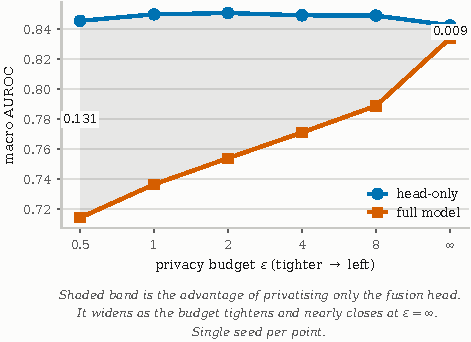
\includegraphics[width=\columnwidth]{fig8_epsilon.pdf}
\caption{Decomposing the recipe across the budget on the clinical corpus. The
shaded band is the initialization effect, obtained with the privatized subset
held at the whole network, and it is nearly the entire advantage. The two
pretrained arms nearly coincide at every budget, although one privatizes $3.3$
times as many parameters as the other, which excludes an explanation based on
privatized dimensionality. Three seeds per point.}
\label{fig:epsilon}
\end{figure}

\subsubsection{Records per individual}
\label{sec:results:kscaling}
Because a patient-level guarantee bounds the \emph{summed} contribution of an
individual, its cost is expected to increase with the number of records per
individual and to vanish when each individual contributes a single record.
Table~\ref{tab:kscaling} reports both arms as $k$, the number of training
records retained per patient, is varied over $\{1, 2, 4, 8\}$ with three seeds.
The number of units sampled per step is equal in both arms, which removes the
sampling-rate effect, so only the clipping geometry differs. The validation and
test partitions are unchanged.

\begin{table}[!t]
\centering
\caption{Average precision by records per individual $k$. The gap is paired by
seed and reported as mean $\pm$ the half-width of a Student-$t$ interval over
three seeds; an interval excluding zero is one whose half-width is smaller than
its mean.}
\label{tab:kscaling}
\setlength{\tabcolsep}{4pt}
\begin{tabular}{ccccc}
\toprule
$k$ & Record & Individual & Gap & $p$ \\
\midrule
$1$ & $0.5015$ & $0.5067$ & $-0.0052 \pm 0.0613$ & $0.7514$ \\
$2$ & $0.5590$ & $0.5084$ & $0.0507 \pm 0.0090$ & $0.0017$ \\
$4$ & $0.5924$ & $0.5092$ & $0.0832 \pm 0.0138$ & $0.0015$ \\
$8$ & $0.5955$ & $0.5089$ & $0.0866 \pm 0.0263$ & $0.0049$ \\
\bottomrule
\end{tabular}
\end{table}

At $k = 1$, the two arms are indistinguishable, with a gap of $-0.0052$ and an
interval covering zero, as required by the construction. The divergence at
larger $k$ can therefore be attributed to the privacy unit rather than to the
experimental setup. From $k = 2$ onward, the gap is resolved and increases
monotonically, reaching $0.0866$ at $k = 8$; the increment from $k = 4$ to
$k = 8$ is an order of magnitude smaller than the preceding one.

The individual-level arm remains flat in $k$, within $[0.4967, 0.5176]$ across
all configurations, whereas the record-level arm increases from $0.5015$ to
$0.5955$. The widening gap therefore reflects a lack of improvement under the
stricter unit rather than a degradation. Additional records per patient provide
signal that the record-level arm exploits and the individual-level arm cannot,
because the bound on the summed contribution is tightest for the individuals
who contribute the additional records. On this corpus, collecting more data per
patient therefore increases the relative cost of an individual-level guarantee.

The area under the ROC curve changes in the same direction, by $0.0006$,
$0.0094$, $0.0133$ and $0.0132$ over the same values of $k$, but every interval
covers zero at three seeds. The effect is therefore resolved in average
precision only. Accuracy is not reported for these arms, because an
uncalibrated decision threshold on an imbalanced corpus keeps it near the
majority rate; an area under the ROC curve of approximately $0.835$ confirms
that the models rank well.

% --- external replication of the k-law, and its matched-budget control ----
% Both are \subsubsection fragments and belong inside
% \subsection{The Privacy Unit and the Budget}, beside "Records per
% individual" above. Keep them in this order: the second explains a confound
% in the first.
%==============================================================================
% results_kscaling_eicu.tex — external validation of the records-per-individual
% law on eICU-CRD. MERGED: \input from results.tex after "Records per
% individual" (sec:results:kscaling).
%
% Every number below is read from an artifact:
%   results/phase5/k_scaling/eicu/k{K}_seed{S}/hist_{arm}_test.json
%       -> auprc (primary), macro_auc (secondary)
%   results/phase5/k_scaling/eicu/k_scaling_eicu.csv   (collected summary)
%   document/01_planning/PREREGISTRATION_EICU.md       (frozen forecast, §2;
%                                                       amendment A1)
%   data/processed/eicu/meta/dataset_meta.json         (corpus description)
%
% k = 16 COMPLETE at three seeds as of 21 September 2026; the row is in the
% table and P1c is settled below. Per-seed gaps +0.0146, +0.0222, -0.0054.
%==============================================================================

\subsubsection{External validation of the records-per-individual law}
\label{sec:results:kscaling:eicu}

The law of Section~\ref{sec:results:kscaling} was measured on a single corpus
whose clients are surgical specialties rather than institutions, so it is not
established whether it characterizes patient-level private federated learning
in general or only that cohort. It is therefore tested on a second clinical
corpus of different construction: $3{,}782{,}805$ hourly windows from
$132{,}736$ individuals across $187$ clients that are \emph{real hospitals},
with a median of $444$ individuals per client and $28.50$ records per
individual. The label is in-unit mortality, with a prevalence of $0.0422$.

Two properties of this replication are relevant. First, its encoders were
pretrained on $526{,}867$ windows verified to be disjoint from every client's
training data, so the results do not carry the oracle-configuration caveat that
applies elsewhere in this paper. Second, the prediction was fixed before the
corpus was constructed. Fitting the four VitalDB points of
Table~\ref{tab:kscaling} gives
\begin{equation}
\mathrm{gap}(k) = A\left(1 - e^{-b(k-1)}\right),
\label{eq:kcurve}
\end{equation}
with $A = 0.0878 \pm 0.0035$ and $b = 0.883 \pm 0.129$ at a root-mean-square
error of $0.0028$. This curve, together with an acceptance band of $\pm 0.030$
derived from the VitalDB seed spread, was registered before any record of the
second corpus was accessed.

\begin{table}[!t]
\centering
\caption{Average precision by records per individual $k$ on the external
corpus, three seeds, paired by seed. Intervals are Student-$t$ half-widths as
elsewhere. The row $k = 16$ lies beyond the range of the first corpus. The final column is
the value predicted by Eq.~\eqref{eq:kcurve}, fixed before the corpus was
built.}
\label{tab:kscaling_eicu}
\setlength{\tabcolsep}{4pt}
\begin{tabular}{cccccc}
\toprule
$k$ & Record & Individual & Gap & $p$ & Predicted \\
\midrule
$1$ & $0.2105$ & $0.2212$ & $-0.0107 \pm 0.0211$ & $0.1594$ & $0.0000$ \\
$2$ & $0.2245$ & $0.2185$ & $+0.0060 \pm 0.0100$ & $0.1215$ & $0.0515$ \\
$4$ & $0.2318$ & $0.2208$ & $+0.0110 \pm 0.0714$ & $0.5746$ & $0.0816$ \\
$8$ & $0.2374$ & $0.2239$ & $+0.0135 \pm 0.0592$ & $0.4296$ & $0.0876$ \\
$16$ & $0.2363$ & $0.2258$ & $+0.0105 \pm 0.0354$ & $0.3310$ & $0.0878$ \\
\bottomrule
\end{tabular}
\end{table}

The control holds. At $k = 1$, the gap is $-0.0107$, with an interval covering
zero and a magnitude within the pre-specified tolerance of $0.020$. The two arms
are therefore not separated where the construction requires them to agree, and
the remaining rows can be attributed to the privacy unit.

The point forecasts are not confirmed. At every $k > 1$, the gap lies outside
the $\pm 0.030$ band, and the measured cost is approximately one sixth of the
predicted cost: $0.0135$ against $0.0876$ at $k = 8$.

Two properties of the law are reproduced. The first is the ordering: the gap is
negative at $k = 1$, positive at $k = 2$, and increases through $k = 4$ to
$k = 8$, as described by Eq.~\eqref{eq:kcurve}. This is consistent with the
mechanism, since the bound on an individual's summed contribution is tightest
for individuals who contribute additional records.

The second is the saturation, which the first corpus cannot test. The
registered prediction was that the gap beyond $k = 8$ would exceed the gap at
$k = 8$ by less than $0.015$. Across paired seeds, the increment from $k = 8$ to
$k = 16$ is $-0.0030$, with an interval of $[-0.0316, +0.0255]$ ($p = 0.692$).
The gap does not continue to increase, and the registered bound is met. The
cost of the guarantee therefore approaches a ceiling in $k$ on both corpora.

The asymmetry between the arms is also reproduced. Across all $k$, the
individual-level arm varies within $[0.2185, 0.2258]$, a range of $0.0073$
against the pre-specified $0.020$, whereas the record-level arm increases from
$0.2105$ to $0.2374$. As on the first corpus, the widening gap reflects
improvement of the record-level arm rather than degradation of the
individual-level arm. The corpora therefore differ in the magnitude of the
effect but not in its mechanism, and, as registered in advance, the shape is
interpreted as structural and the magnitude as corpus-dependent.

The statistical power of this replication is limited. At three seeds, no gap in
Table~\ref{tab:kscaling_eicu} is resolved: every interval covers zero, and no
$p$-value is below $0.12$. The seed standard deviation of the gap at $k = 8$ is
of the same order as the gap, and resolving an effect of this size at
conventional power would require approximately fifty seeds, against the three
fixed in advance. The seed count was not increased after inspecting the
results. The trend is therefore reported as directionally consistent with the
VitalDB law and unresolved on this corpus. The area under the ROC curve is
less informative: its gaps over the same values of $k$ are $-0.0012$,
$-0.0015$, $+0.0018$, $+0.0001$ and $+0.0105$, with no trend over the range
covered by the first corpus. Average precision is the primary measure on this
corpus, as on the first, and the area under the ROC curve provides no evidence
either way.

One possible explanation for a preserved shape at a lower ceiling is offered as
a hypothesis. The two tasks differ in attainable precision by approximately a
factor of two: the arms on this corpus lie within $[0.1960, 0.2446]$ at a
prevalence of $0.0422$, whereas those on the first corpus lie between $0.4967$
and $0.5955$. A gap in average precision is bounded by the attainable
precision, so a cost that is a fixed fraction of attainable performance would
produce a smaller absolute gap on the harder task with the same ordering in
$k$. Under this explanation, the transferable quantity is the cost relative to
attainable precision rather than the ceiling $A$. Distinguishing this from a
corpus-specific ceiling requires a third corpus.

The range of $k$ is limited by the corpus. The registered design specified $k$
up to $32$. On this corpus, however, a budget of twenty-four windows per
admission means that only $20.2\,\%$ of individuals reach thirty-two records,
and these individuals have multiple admissions and are not representative of
the cohort. Estimating the arm at $k = 32$ would therefore measure the effect
of readmission rather than of the privacy unit. The maximum was reduced to
$16$, which retains $91.0\,\%$ of individuals, and $k = 32$ is reported as
untested. This change was recorded as a dated amendment to the registration
before any result beyond $k = 8$ was computed, and it did not alter any
predicted value.

%==============================================================================
% COMPLETE. k = 16 landed 21 September 2026 at three seeds; P1c is settled in
% the body above. No pending artifact remains for this subsection.
%   artifacts : results/phase5/k_scaling/eicu/k_scaling_eicu.csv (30 rows)
%               results/phase5/k_scaling/eicu/k{1,2,4,8,16}_seed{42,43,44}/
%   k = 32 is reported UNTESTED, not dropped — amendment A1.
%==============================================================================

%==============================================================================
% results_a2_budget.tex — matched-budget control for the external test.
%
% MERGED: \input from results.tex immediately after
% sections/results_kscaling_eicu.tex. It is a \subsubsection and sits inside
% \subsection{The Privacy Unit and the Budget}.
%
% Every number is read from an artifact:
%   results/phase5/k_scaling/a2_matched_budget.json   (written by
%     scripts/analyze_k_matched.py, which resolves each grid's budget from the
%     argv recorded in its run_metadata_*.json — nothing is hardcoded)
%   results/phase5/k_scaling/vitaldb/k_scaling_vitaldb.csv        eps_train 1.00
%   results/phase5/k_scaling/vitaldb_eps080/k_scaling_vitaldb.csv eps_train 0.80
%   results/phase5/k_scaling/eicu/k_scaling_eicu.csv              eps_train 0.80
%   document/01_planning/PREREGISTRATION_EICU.md  amendment A2
%==============================================================================

\subsubsection{A matched-budget control for the external test}
\label{sec:results:kscaling:a2}

The comparison of the two preceding subsubsections is confounded by the
training budget. The curve of Eq.~\eqref{eq:kcurve} was \emph{fitted} on a
first-corpus grid trained at $\varepsilon_{\mathrm{train}} = 1.00$ and
\emph{tested} on a second-corpus grid trained at
$\varepsilon_{\mathrm{train}} = 0.80$, the operating point of
Section~\ref{sec:experiments}. Since additional noise reduces the difference
between any two arms, which is the same direction as the observed shortfall,
the shortfall cannot be attributed to the corpus without a control.

The pre-registered correction re-runs the first corpus at the operating point
of the second, with $k$, seeds, partitions and protocol unchanged, and without
refitting the forecast. Table~\ref{tab:kscaling_matched} compares the three
grids.

\begin{table}[!t]
\centering
\caption{Average precision gap (record arm minus individual arm, paired by
seed, three seeds) across the three grids. The first two differ only in the
training budget. The forecast column is Eq.~\eqref{eq:kcurve}, fitted on the
first column and never refitted.}
\label{tab:kscaling_matched}
\setlength{\tabcolsep}{3.5pt}
\begin{tabular}{ccccc}
\toprule
 & Forecast & First corpus & First corpus & Second corpus \\
$k$ & & $\varepsilon_{\mathrm{tr}}\!=\!1.00$ & $\varepsilon_{\mathrm{tr}}\!=\!0.80$ & $\varepsilon_{\mathrm{tr}}\!=\!0.80$ \\
\midrule
$1$ & $0.0000$ & $-0.0052$ & $+0.0380$ & $-0.0107$ \\
$2$ & $0.0515$ & $+0.0507$ & $+0.0355$ & $+0.0060$ \\
$4$ & $0.0816$ & $+0.0832$ & $+0.0945$ & $+0.0110$ \\
$8$ & $0.0876$ & $+0.0866$ & $+0.0967$ & $+0.0135$ \\
\bottomrule
\end{tabular}
\end{table}

Taken at face value, the budget explains almost none of the shortfall. The
matched gaps are not smaller than the original ones: at $k = 8$, the matched gap
is $+0.0967$ against $+0.0866$, so the lower budget moved the first corpus in
the \emph{opposite} direction to that predicted by the confound. Decomposing the
total change at $k = 8$ attributes $+0.0101$ to the budget and $-0.0832$ to the
corpus.

Two qualifications apply. First, the re-run did not change the budget alone:
the operating point also changes the batch size from $32$ to $64$ units, so the
budget term is the joint contribution of the budget and the sampling
configuration. Second, the matched grid fails its own positive control. At
$k = 1$, where the two arms must agree by construction, it separates them by
$+0.0380$, with all three seeds of the same sign, against a pre-specified
tolerance of $0.020$. The interval covers zero, so the result is formally
unresolved, but the consistent sign is notable, and both the original grid
($-0.0052$) and the external grid ($-0.0107$) pass the same check.

The failure is attributable to the sampling configuration rather than to the
budget. At $k = 1$, the first corpus retains one record per individual, giving
a training pool of $4{,}372$ records, the smallest in this study; with a batch
of $64$, this yields approximately sixty-eight optimization steps per round for
either arm. The original grid uses the same pool with a batch of $32$ and its
control passes, and the external corpus uses $76{,}589$ records with a batch of
$64$, seventeen times more data at the same batch size, and its control also
passes. The failing configuration combines the smallest pool with the largest
batch, which indicates a lack of power rather than an effect of the privacy
unit, consistent with the width of the interval.

Subtracting each grid's own $k = 1$ offset from its other rows gives a
conservative estimate. At $k = 8$, the budget and sampling term then accounts
for $-0.0331$ and the corpus for $-0.0345$; at $k = 4$, for $-0.0320$ and
$-0.0347$. The two contributions are then comparable. Under the face-value
estimate, the budget contributes nothing; under the conservative estimate, it
contributes about half. Under neither does it account for the factor of six
separating the two corpora at $k = 8$, and under neither does the corpus term
change sign. The matched grid therefore shows that the budget mismatch cannot
account for the external shortfall, but not that the mismatch contributed
nothing.

The control failure is confined to this re-run. The scaling law of
Table~\ref{tab:kscaling} and its external test in
Table~\ref{tab:kscaling_eicu} are measured on grids whose $k = 1$ controls
pass, so neither depends on the grid reported here; only the decomposition of
the difference between them does. The matched grid is therefore reported as a
bound on a confound rather than as a measurement.


\subsubsection{Is the cost an artifact of the clipping rule?}
\label{sec:results:kscaling:nd}

% Artifacts:
%   results/phase5/nd_clipnorm/eicu/nd_clipnorm_eicu_natural.json  (9 runs)
%   results/phase5/nd_clipnorm/eicu/hist_natural_seed*_*.csv       saturation
%   results/phase5/nd_clipnorm/eicu/clip_saturation_natural_seed42.json
%   document/01_planning/PREREGISTRATION_ND_CLIPNORM.md  amendments N-A1, N-A2

The individual-level arm clips each individual's \emph{summed} gradient to a
fixed norm, so clipping is strongest for individuals with many records. The
flatness of this arm in $k$ could therefore result from the clipping rule
rather than from the guarantee. In that case, it should be partly recoverable
by dividing the summed gradient by the record count, or by its square root,
before clipping. Neither normalization changes the guarantee: sensitivity is
determined by the clipping norm, so the noise scale and the budget are
identical under all three rules, and any difference is due to optimization.

The premise holds in direction but not in magnitude. On the external corpus,
the fraction of individuals whose gradient is clipped increases from $0.148$
for those with one to four records to $0.502$ for those with forty-nine or
more, but the rank correlation between record count and clipping is only
$0.138$. Normalizing by the count halves the clipped fraction, from $0.3945$ to
$0.2039$, rather than eliminating it. The first corpus cannot test this
question, because nearly every individual contributes exactly eight records, so
normalization by the count is a uniform rescaling. The test is therefore
performed on the external corpus only, using its natural partition rather than
the capped partitions of the scaling grid, since capping would remove the
variation in records per individual, which ranges from two to $192$.

Normalization does not recover utility. At the operating budget and three
pre-specified seeds, the individual-level arm attains an average precision of
$0.2266$ with the fixed bound, $0.2265$ with normalization by the count, and
$0.2242$ with normalization by its square root. The paired differences relative
to the fixed bound are $-0.0001 \pm 0.0087$ and $-0.0024 \pm 0.0095$. The
pre-registered threshold for recovery was $+0.010$ for normalization by the
count, obtained by scaling the threshold for the first corpus to the precision
attainable on this corpus. The one-sided $95\,\%$ upper bound on the difference
is $+0.0058$, so an effect of the registered size is excluded. The area under
the ROC curve changes in the same direction, by $-0.0022$ and $-0.0011$. The
square-root rule, predicted to fall between the other two, falls below both,
although by less than the seed variation.

The intervention was effective: from the third round onward, on every seed,
normalization by the count produced the lowest clipped fraction and the fixed
bound the highest. In the final round, the fractions are $0.157$ against
$0.212$ on one seed, and $0.046$ against $0.086$ and $0.047$ against $0.118$ on
the others. On one seed, the selected checkpoint for every rule is the first
round, before the rules diverge, so the three rules agree to within $10^{-4}$
and this seed carries little information about the contrast. The cost of the
individual-level unit is therefore not an artifact of the clipping rule.

\subsection{Does Fusion Earn Its Place?}
\label{sec:results:fusion}

The benefit of combining the two modalities is evaluated separately from the
federated system, because the question concerns the data rather than the
protocol, and federation and privacy noise would add variance and confounds.
Each arm is retrained on its own inputs rather than evaluated with one modality
zeroed, since zeroing a stream of a jointly trained model measures robustness
to a missing stream rather than the information it carries.

Over five seeds, the fused model attains $0.8653 \pm 0.0072$ in area under the
ROC curve, against $0.8283 \pm 0.0087$ for the better single modality and
$0.7680 \pm 0.0045$ for the weaker, where each interval is a Student-$t$
half-width. The gain of $0.0370$ is $5.9$ times the seed standard deviation,
and the gain in average precision is $0.0671$. The modalities are paired by the
recording apparatus, from the same patient during the same operation, so the
gain does not arise from a pairing rule. With two seeds, the same experiment
gave gains of $0.0411$ and $0.1062$, at $14.1$ times the seed standard
deviation; with five seeds, the average-precision gain is $37\,\%$ lower and
the effect size less than half as large. Only the five-seed values are used.

On the wearable deployment, the better single modality already attains
$0.9976$, leaving a fusion gain of $0.0004$ and no room for a second stream to
contribute. The benefit of fusion therefore depends on the task and must be
established per task.

\subsubsection{The external clinical corpus, and the condition that separates
the three}
\label{sec:results:fusion:balance}

% Artifacts (every number below is read from these; nothing is hand-entered):
%   results/phase5/ablation_eicu.json            full client data, the quoted null
%   results/phase5/ablation_eicu_matched.json    matched control, current partitions
%   results/phase5/ablation_eicu_noapache.json   Stage 1, dominant channel zeroed
%   results/phase5/fusbal_calib_n{0.20..0.80}.json  calibration, arm B only
%   results/phase5/fusbal_test_n0.4.json         the registered test, 5 seeds
%   document/01_planning/PREREGISTRATION_FUSION_BALANCE.md  amendment F-A1

On the external clinical corpus, which has more headroom than the wearable
corpus, fusion yields no gain. The fused model attains $0.8249$ in area under
the ROC curve against $0.8212$ for the admission-record stream alone, a gain of
$0.0037$, and $-0.0001$ in average precision. The vital-sign stream alone
reaches $0.6748$, so the two streams differ substantially in strength. This
motivates a second hypothesis, that fusion requires the streams to be of
comparable strength, which was pre-registered before testing.

The test weakens the stronger stream until the two are balanced and measures
whether a gain appears. Zeroing the dominant admission feature reversed the
dominance rather than balancing the streams (Table~\ref{tab:fusion_balance}).
Scaling the feature was ineffective, because the stream is standardized and its
encoder is linear at the input, so scaling is compensated by the weights; a
scale of $0.15$ changed the stream by $0.0007$. The intervention used therefore
mixes the feature with fixed-seed Gaussian noise at a ratio that preserves its
variance, which removes information rather than rescaling it. A calibration on
the admission stream alone, with two seeds, changed its performance
monotonically from $0.6252$ to $0.7859$ across four mixing levels, and the level
closest to the vital-sign stream was selected. Because the calibration uses only
one single-modality arm and never the fused model, it does not select on the
outcome. Because the current partitions contain $20\,\%$ less client data than
the run reported above, the comparator was re-measured on them; its gain of
$0.0020$ confirms that the reduction does not affect the null result.

\begin{table}[!t]
\centering
\caption{Fusion on the external clinical corpus as the stronger stream is
weakened. Area under the ROC curve, mean over five seeds in every row; gains
are over the better single modality, in area under the ROC curve and in
average precision (AP).}
\label{tab:fusion_balance}
\setlength{\tabcolsep}{3.2pt}
\begin{tabular}{lccccc}
\toprule
Condition & Vitals & Admission & Fused & Gain & Gain (AP) \\
\midrule
Matched control  & $0.7068$ & $0.8221$ & $0.8241$ & $+0.0020$ & $-0.0008$ \\
Feature zeroed   & $0.6973$ & $0.5947$ & $0.6911$ & $-0.0062$ & $-0.0182$ \\
Titrated to parity & $0.6992$ & $0.6845$ & $0.7282$ & $\mathbf{+0.0291}$ & $+0.0121$ \\
\bottomrule
\end{tabular}
\end{table}

When the streams are balanced, a gain appears. With the two single-modality arms
within $0.0147$ of each other, the fused model attains $0.7282 \pm 0.0191$
against $0.6992 \pm 0.0120$ for the better single modality, a gain of
$0.0291 \pm 0.0211$. The gain is positive on all five seeds, with a minimum of
$0.0129$ (paired $t$-test, $p = 0.019$; the signed-rank test gives
$p = 0.0625$, its minimum attainable value at five seeds). The result exceeds
the pre-registered threshold of $0.015$ and is fourteen times the gain of the
matched control. In average precision, the gain is $0.0121 \pm 0.0215$, with one
negative seed, and is not resolved.

The scope of this result is limited in two respects. Balance was imposed by
calibration, so the result shows that comparable stream strength is
\emph{sufficient} for a fusion gain on this corpus, but not that it is
necessary. In addition, the gain is measured against a deliberately weakened
stream: the balanced fused model remains well below the intact admission
stream, so the result does not support fusing the two streams in the deployed
configuration.

\subsection{Necessity of the Components}
\label{sec:results:ablation}

Each component is removed in turn from the full system, with all other settings
fixed, and the arms are paired by seed over three seeds
(Table~\ref{tab:ablation}). Of the four removals, only the removal of the
privacy mechanism produces an interval that excludes zero.

\begin{table}[!t]
\centering
\caption{Component ablation on the clinical deployment. $\Delta$AUROC is paired
against the full system by seed over three seeds, reported as mean $\pm$ the
half-width of a Student-$t$ interval; an interval excludes zero when the
half-width is smaller than the mean, and the one that does is set in bold. MB is
the total compressed payload uploaded across training. C6 is an
\emph{inclusion} arm: for it a rise, not a fall, would indicate a contribution.}
\label{tab:ablation}
\small
\setlength{\tabcolsep}{3pt}
\begin{tabular}{llcr}
\toprule
Removed & AUROC & $\Delta$AUROC & MB \\
\midrule
--- (full)        & $0.8541$ & ---                  & $252$ \\
C1 hierarchy      & $0.8484$ & $-0.0058 \pm 0.0088$ & $50$ \\
C2 privacy        & $0.8307$ & $\mathbf{-0.0234 \pm 0.0205}$ & $252$ \\
C3 sparsification & $0.8553$ & $+0.0012 \pm 0.0083$ & $1260$ \\
C4 quantization   & $0.8543$ & $+0.0001 \pm 0.0006$ & $403$ \\
+C6 ASWA          & $0.8542$ & $+0.0001 \pm 0.0009$ & $252$ \\
\bottomrule
\end{tabular}
\end{table}

\subsubsection{Compression is justified by traffic, not by accuracy}
Removing top-$\kappa$ sparsification changes the area under the ROC curve by
$+0.0012$, with an interval spanning zero, and increases uplink traffic by a
factor of $5.0$. Removing quantization changes it by $+0.0001$, with an
interval of width $0.0011$, the narrowest in the study, and increases uplink
traffic by a factor of $1.60$. Neither component affects predictive
performance; together they reduce the payload eightfold at no measurable cost
in discrimination.

\subsubsection{The edge tier does not cost accuracy}
Removing the edge tier changes the area under the ROC curve by $-0.0058$ at
three seeds, with an interval covering zero. With the six seeds specified in
the pre-registration, the effect is resolved on both deployments: $-0.0047$
$[-0.0088, -0.0006]$ ($p = 0.032$) on the clinical corpus and $-0.0052$
$[-0.0074, -0.0030]$ ($p = 0.0018$) on the wearable corpus. Removing the tier
therefore slightly reduces performance.

This result is interpreted as a bound on the cost of the hierarchy rather than
as a benefit, because the flat arm differs in two respects. It uses a single
edge with one edge round per global round, whereas the hierarchical arm uses
five, so it changes both the aggregation schedule and the topology. The small
advantage may be due to the additional aggregation steps rather than to the
tier itself; separating the two would require a flat arm matched on
aggregation steps. For the same reason, the uplink value of this arm is not
comparable with the others. The comparison shows that the edge tier does not
reduce predictive utility, so the communication and energy savings of
Section~\ref{sec:results:objectives} are not obtained at the expense of
accuracy.

\subsubsection{Removing the privacy mechanism does not recover utility}
Training the same system without differential privacy \emph{reduces} the area
under the ROC curve by $0.0234$ $[-0.0439, -0.0029]$ and increases the
seed-to-seed spread in average precision from $\pm 0.014$ to $\pm 0.070$. Two of
the three non-private seeds reach their best validation score in the first of
ten rounds and degrade thereafter, whereas every private seed peaks between
rounds six and nine. Clipping and calibrated noise therefore act as a
regularizer for a compact head trained over frozen features, and without them
the head overfits early.

This comparison is against a baseline without additional regularization beyond
checkpoint selection, not against a non-private system tuned for
generalization, which would typically use weight decay or early stopping. The
result shows that removing the guarantee does not recover utility on this task;
it does not show that differential privacy improves accuracy in general. It
also shows that the accuracy cost of the guarantee, bounded at two percentage
points in Table~\ref{tab:results_objectives}, is not incurred at this operating
point.

\subsubsection{Loss-aware edge weighting}
The aggregation rule ASWA, inherited from an earlier version of this framework,
weights each edge at the cloud by both its data volume and the mean local loss
of its clients, instead of by data volume alone. It was evaluated as an
inclusion arm. Adding it to the full system changes the
area under the ROC curve by $+0.0001$, with an interval of width $0.0018$ that
covers zero, and leaves uplink traffic unchanged. Since this is an inclusion
arm, an increase would indicate a contribution, and none is observed. The
component is therefore not adopted.

\subsection{Membership-Inference Audit}
\label{sec:results:mia}

Table~\ref{tab:mia} reports the empirical leakage of three configurations
under both attacks of Section~\ref{sec:method:mia}. Each attack uses sixteen
shadow models trained on independently sampled halves of the patient
population, and each configuration is scored on the same $600$ member and
$600$ non-member patients.

\begin{table}[!t]
\centering
\caption{Patient-level membership inference. Mean attack AUC over seeds with
$95\,\%$ intervals; $0.5$ is chance. The control is non-private training of the
same head over the same frozen encoders.}
\label{tab:mia}
\small
\setlength{\tabcolsep}{4pt}
\begin{tabular}{llcc}
\toprule
Configuration & Attack & AUC & 95\,\% CI \\
\midrule
Control (non-private) & lik.\ ratio & $0.6230$ & $[0.598, 0.648]$ \\
Record-level DP       & lik.\ ratio & $0.5477$ & $[0.488, 0.608]$ \\
Patient-level DP      & threshold   & $0.5224$ & $[0.518, 0.527]$ \\
\bottomrule
\end{tabular}
\end{table}

The positive control confirms that the audit can detect leakage. On non-private
training of the same head over the same frozen encoders, the likelihood-ratio
attack reaches $0.6230$, compared with $0.5711$ for loss thresholding.
Per-patient calibration thus recovers $0.0519$ of signal that a global
threshold misses because of per-patient difficulty, as illustrated in
Fig.~\ref{fig:lira}.

The strength of the control does not depend on training length. Training for
ten rounds instead of one changes the likelihood-ratio attack by $-0.0047$, and
no attack by more than $0.006$. A head of $560$k parameters over frozen
encoders therefore reaches its memorization capacity almost immediately, and a
stronger control would require a different configuration rather than longer
training.

On the private configurations, leakage is low. Record-level differential
privacy yields $0.5477$, with an interval that includes chance, and
patient-level differential privacy yields $0.5224$. The primary comparison, the
paired difference between the two over five seeds on identical shadow splits,
is not significant under any of the four attacks: $+0.0138$
$[-0.0034, +0.0310]$ for the loss threshold, $+0.0325$ $[-0.0280, +0.0929]$ for
the offline likelihood ratio, $+0.0034$ for the online variant and $-0.0211$
for its pooled-variance form. All intervals span zero.

The \emph{predicted} effect is therefore refuted. The hypothesis was that a
record-level guarantee would be exploitable at the individual level, with an
attack AUC approaching $0.7$ against approximately $0.5$ for a patient-level
guarantee, and an effect of this size lies outside every interval obtained. A
\emph{small} effect is not excluded: at five seeds, the half-width for the
strongest attack is $\pm 0.060$, three of the four attacks point in the
predicted direction, and the loss threshold reaches $p = 0.090$. The large
predicted effect is thus absent, and an effect below approximately six points
of AUC cannot be resolved at this sample size. The two guarantees cannot be
considered equivalent on this evidence.

On the patient-level arm, the likelihood ratio performs \emph{worse} than the
loss threshold, by $0.0071$. Since per-patient calibration helps only when
difficulty-confounded signal is present, its benefit on the control and its
absence on the patient-level arm indicate that the defense leaves little such
signal. True-positive rates at a $1\,\%$ false-positive rate are low, at
$0.029$ on the control and $0.010$ on the patient-level arm. At $0.1\,\%$, the
rate is undefined, because $600$ non-members are insufficient to resolve this
false-positive rate.

The analytic argument of Section~\ref{sec:method:threat} therefore stands: a
record-level budget bounds the wrong quantity, and its conversion to an
individual-level budget is prohibitive, while the utility cost of enforcing the
individual-level guarantee directly is small. The audit does not, however,
show that the weaker guarantee is exploitable in practice on this data at this
budget.

% FLOAT PLACEMENT NOTE: fig7_energy is declared near the TOP of this section,
% not beside the Energy subsection that discusses it. A figure* can only be set
% at a page top, and declared at its point of discussion — the last subsection
% of the last section — the only page top LaTeX could still reach was the one
% the bibliography starts on, stranding it after the references. Declaring a
% double-column float one or two pages of text ahead of its citation is the
% standard remedy; LaTeX never places a float before its declaration.
%==============================================================================
% PENDING SUBSECTIONS — experiments not yet complete. Add each only when its
% artifact exists; do not pre-write numbers.
%
%   (Multimodal fusion ablation: COMPLETE 2026-08-16 at n=5, written up at
%    \label{sec:results:fusion}. +0.0370 AUROC / +0.0671 AUPRC, 5.9x seed-sd.
%    The n=2 figures were seed-lucky and are archived at
%    results/phase5/archive_fusion_2seed/. Quote five-seed only.)
%
%   (Component ablation: COMPLETE 2026-08-17 at n=3 seeds, written up at
%    \label{sec:results:ablation}. Only C2 resolves. Artifacts:
%    results/phase6/vitaldb/ablation_A*_seed*.json)
%
%   (MIA control: re-run 2026-08-17 after the --no_dp early-stop fix; the
%    published control had trained 1 round of 10. lira_offline 0.6277 -> 0.6230,
%    i.e. essentially unchanged. Prior artifacts archived under
%    results/phase5/lira/vitaldb/*_1round_*.)
%
%==============================================================================

%==============================================================================
% discussion.tex — Discussion for PP-HFM
% Self-contained \section{}; \input this into main.tex (never compile alone).
%
% STATUS: PARTIAL. Only the Limitations subsection is written. The interpretive
% subsections are deliberately withheld until Results is complete, because
% three of their arguments are still undetermined:
%   - whether the cost of the privacy unit scales with records per individual
%     (records-per-individual experiment, running)
%   - whether every component earns its place (component ablation A1--A4,
%     never run)
%   - whether the fusion gain survives more seeds  [RESOLVED 2026-08-16: it
%     does, at n=5, but shrank from +0.0411/+0.1062 to +0.0370/+0.0671 and
%     from 14.1x to 5.9x seed-sd. Quote the five-seed figures only.]
% Writing the interpretation against a half-populated Results guarantees a
% rewrite. Every limitation below is settled and will not move.
%==============================================================================

\section{Discussion}
\label{sec:discussion}

\subsection{Limitations}
\label{sec:discussion:limits}

The claims of this paper are bounded in ways that are worth stating precisely,
because several of them constrain what may be generalised from the results
rather than merely qualifying them.

\textbf{The privacy-unit results are single-domain, for a structural reason.}
The framework is evaluated on two corpora, but the measurements concerning the
unit of the guarantee are reported only on the clinical one. This is not an
oversight of scope. In the wearable corpus each client corresponds to exactly
one participant, so client-level, user-level and individual-level guarantees
coincide and the divergence the mechanism addresses cannot arise there. A
second corpus exhibiting the same many-individuals-per-client structure --- a
second clinical cohort, or an institutional deployment in another domain ---
would be required to establish that the measured cost transfers, and its
absence is the most predictable objection to this work.

\textbf{The fusion result is single-domain, and the second corpus cannot
corroborate it either.} The gain from combining the modalities is established
on the clinical cohort, where it reaches $0.0370$ in area under the ROC curve
over the better single modality across five seeds, or $5.9$ times the seed
standard deviation. It is not established on the wearable cohort, and the
reason is a property of that task rather than of the framework: its better
single modality already attains $0.9976$, leaving a gain of $0.0004$ and no
headroom in which fusion could demonstrate anything. This is worth reporting
rather than omitting, because it qualifies the premise the framework is built
on. Multimodal federated learning is not universally motivated; on tasks a
single modality already solves, the second stream adds cost without adding
information, and the case for fusion must be made per task rather than assumed
from the presence of two sensors. Establishing that the measured gain transfers
would require a second corpus that is both genuinely paired at source and
difficult enough to leave room for the second modality to matter --- the same
requirement, and the same absence, as for the privacy-unit results above.

\textbf{Reported utilities come from the oracle encoder configuration.} As
Section~\ref{sec:exp:impl} records, the encoders behind the reported results
were pretrained on the pooled client training data, which does not carry a
valid end-to-end guarantee. The deployable configuration costs $0.0322$ in
area under the ROC curve, and every absolute utility in this paper should be
read as an upper bound on what it attains. The differences between arms, on
which the claims rest, are unaffected because every arm shares the same
encoders; but a reader comparing these figures against a system that respected
disjointness throughout would not be comparing like with like.

\textbf{The membership-inference null bounds a large effect only.} The audit
establishes that the difference in leakage between a record-level and an
individual-level guarantee is not of the magnitude hypothesised. It does not
establish that the difference is zero. At five paired seeds the half-width on
the strongest attack is $\pm 0.060$ in area under the curve, three of the four
attacks point in the predicted direction, and the strongest of them reaches
$p = 0.090$; an effect below roughly six points would be invisible to this
design. The result should be cited as a refutation of the predicted effect,
never as evidence that the two guarantees are equivalent.

\textbf{The audit rests on sixteen shadow models.} Per-individual in- and
out-distributions are estimated from roughly eight observations each, which is
few for a variance estimate and is the reason a pooled-variance variant is
reported alongside the per-individual one. A larger shadow population would
tighten those fits and is the first thing to increase if the audit were to be
repeated. Relatedly, with $600$ non-members the receiver operating
characteristic cannot resolve a $0.1\,\%$ false-positive rate, so the
low-false-positive corner --- which is where a confident disclosure would
appear --- is characterised only at $1\,\%$.

\textbf{One objective is inconclusive and must remain so.} On the wearable
deployment the accuracy cost under the budget is $1.967$ pp with an interval of
$[1.760, 2.173]$, which spans the $2$ pp requirement. The seed count of fifteen
was fixed in advance, and extending it until the interval fell on the
favourable side of the threshold would convert a pre-registered test into a
search. The objective is therefore reported as undetermined rather than as
either met or failed.

\textbf{Several supporting measurements rest on few seeds.} The privacy-budget
sweep of Fig.~\ref{fig:epsilon} is single-seed at each point, so the claim it
supports is the monotonicity of the trend rather than any individual value.
The aggregation-rule comparison that led to a component being dropped was
likewise decided on one seed; the effect was small enough that additional
seeds were judged unlikely to change the decision, but that judgement is not a
measurement.

\textbf{The network model simulates the network only.} Communication delay,
delivery reliability and traffic volume are measured on a packet-level
simulation of the topology, but the compute terms that enter the end-to-end
round latency --- sensing, preprocessing, inference and aggregation --- are
modelled analytically and are common to every topology compared. The
comparison between topologies is therefore sound, since the modelled terms
cancel, but the absolute round latency is not a measurement of a deployed
system and should not be read as one.

\textbf{Interpretability evidence is associational.} The attribution analysis
establishes that the model attends substantially to indicators of whether a
measurement was taken, and that this reliance increases under the privacy
mechanism. It does not establish that the model would lose accuracy without
those indicators, which only their removal could show. The claim is therefore
stated as evidence of reliance, not as a causal contribution to performance.

%==============================================================================
% PENDING SUBSECTIONS — write once Results is complete.
%
%   Interpretation of the privacy-unit cost
%     needs : records-per-individual scaling law (running)
%     turns on whether the cost is a constant of this cohort or a function of
%     records per individual; the second is a far stronger statement
%
%   Necessity of the components
%     needs : component ablation A1--A4 (never run)
%
%   Position against prior art
%     needs : the above, plus the fusion ablation at more than two seeds
%
%   Practical implications for deployment
%==============================================================================

%==============================================================================
% conclusion.tex — Conclusion for PP-HFM.
% Self-contained \section{}; \input this into main.tex (never compile alone).
%
% RULE: no number appears here that does not already appear in Results, and no
% claim is made here that Results does not establish. A conclusion that
% introduces evidence is a conclusion a reviewer reads twice.
%
% The two former [PENDING] sentences -- the fusion condition (amendment F-A1)
% and the clipping-artifact question (amendment N-A2) -- were filled
% 2026-10-21. Results now reports both (sec:results:fusion:balance and
% sec:results:kscaling:nd); they are stated here without numbers regardless.
%
% READABILITY PASS 2026-10-21: sentences split; the N-A2 finding moved from the
% "future directions" paragraph (where it was a result posing as a direction)
% to the paragraph on the cost of the guarantee. Numbers unchanged.
%==============================================================================

\section{Conclusion}
\label{sec:conclusion}

This paper presented a hierarchical federated learning system for multimodal
clinical and wearable sensing that enforces differential privacy at the level
of the individual rather than the record, and quantified the cost of that
choice. On two deployments, the composed budget, including the conformal
calibration release, is $0.970$ and $0.966$. Uplink traffic is reduced by
$90.8\,\%$ and $96.1\,\%$, energy per round by $72.3\,\%$ and $76.8\,\%$, and
the 95th-percentile inference latency is $3.0$ and $1.2$~ms against a
requirement of $100$~ms. Because noise is added to gradients during training,
the privacy mechanism adds no computation at inference.

Two findings are central. First, robustness to a tight privacy budget is
determined by the initialization rather than by the size of the privatized
subset. A pretrained initialization improves on a random one by $0.0187$
without noise and by $0.1447$ at the tightest budget, whereas restricting the
privatized subset contributes at most $0.0036$, with intervals covering zero,
despite privatizing $3.3$ times fewer parameters. The restriction is therefore
justified by its communication savings only.

Second, the cost of an individual-level guarantee increases with the number of
records each individual contributes. At a fixed per-step budget and number of
units per step, the penalty is indistinguishable from zero at one record per
individual and reaches $0.0866$ in average precision at eight, saturating
before that point. Because the two units coincide at one record per
individual, this configuration serves as a built-in control. The
individual-level arm remains flat while the record-level arm improves, so the
cost arises from additional records that the stricter unit cannot exploit.
Normalizing the clipping bound by the record count does not reduce this cost,
which indicates that it is inherent to the unit rather than to the clipping
rule. On a second clinical corpus of $132{,}736$ individuals across $187$
hospitals, the ordering and the saturation transfer, whereas the magnitude is
approximately one sixth of the pre-registered forecast and is not resolved at
three seeds.

Several results are negative. Compression does not affect accuracy and is
justified by traffic reduction alone. An adaptive per-layer allocation of the
budget performs worse than a uniform allocation. The predicted difference in
membership leakage between the two units is not observed under an attack whose
positive control reaches $0.625$. The benefit of multimodal fusion is
conditional: it is $0.0370$ in area under the ROC curve on the first clinical
corpus, untestable on the wearable corpus, where the better single modality
reaches $0.9976$, and absent on the external clinical corpus. A titration on
the external corpus shows that balance between the two streams is a sufficient
condition: when the stronger stream is degraded to parity with the weaker,
fusion yields a significant gain in area under the ROC curve over the better
single modality, although not in average precision and not relative to the
intact stronger stream.

Future work should establish whether the saturation level of the scaling law
is a constant of the guarantee or a fixed fraction of the precision attainable
on a task, which requires a third corpus. Establishing equivalence in leakage
between the two units, rather than the absence of a large difference, requires
a shadow population larger than sixteen and a non-member set large enough to
resolve the low-false-positive regime.

\section*{Data Availability}
VitalDB \cite{ref20} (\url{https://vitaldb.net}) and WEAR \cite{ref21} are
publicly available. The eICU Collaborative Research Database \cite{ref27} is
available through PhysioNet \cite{ref28} to credentialed users under a data
use agreement, so no patient-level records or arrays derived from them are
redistributed. All corpora are de-identified; this study is a secondary
analysis with no patient contact. Code and aggregate results will be released
upon publication.

% Acknowledgment removed at the authors' request (2026-11-04). IEEE policy asks
% for any AI-use disclosure and any funding statement in an Acknowledgment
% section; restore one here if either is needed.


% ---- Bibliography ----------------------------------------------------------
\bibliographystyle{IEEEtran}
\bibliography{references}

\end{document}
